\documentclass[10pt,a4paper]{article}
\usepackage[utf8x]{inputenc}
\usepackage[danish]{babel}
\usepackage{amsmath}
\usepackage{mathtools}
\usepackage{framed}
\usepackage{amsfonts}
%\usepackage{epstopdf}
\usepackage{hyperref}
\usepackage{todonotes}
\usepackage{subfig}
\usepackage{float}
\usepackage{amssymb}
\setlength{\parindent}{0pt}
\usepackage{graphicx}
\usepackage{fullpage}
\DeclarePairedDelimiter\ceil{\lceil}{\rceil}
\DeclarePairedDelimiter\floor{\lfloor}{\rfloor}
\newcount\colveccount
\newcommand*\colvec[1]{
        \global\colveccount#1
        \begin{pmatrix}
        \colvecnext
}
\def\colvecnext#1{
        #1
        \global\advance\colveccount-1
        \ifnum\colveccount>0
                \\
                \expandafter\colvecnext
        \else
                \end{pmatrix}
        \fi
}
\begin{document}
\section{K - means clustering}
Clustering is the task of grouping a set of data points in such a way that data points in the same group (called a cluster) are more similar (in some sense or another) to each other than to those in other groups (clusters).
The clustering is done by minimizing  the sum of square distance between each data point and their corrensponding cluster centroid.  \\

The number of clusters needed  is determined by the user. It usually depends on how the data points  is distributed. Choosing a large number of cluster will result in a reduced squared distance, and indeally zero as each data point gets it own cluster.  The optimal choice of k will consist of having a balance between having the data compressed as possible, and still retain a decent amount of accuracy.  More fomally is the goal to partition the data  into k clusters in order to minimze the total within cluster sum of squares.  For which the elbow method might become handy. \\


\missingfigure{Elbow}

To find the optimal kmeans clustering were figure \textbf{Missing at the moment} used to determine what number of clusters would provide an optimal Total within sum of squared without having to many cluster.  This is found by locating the elbow of the graph, which lies around 30. 

Figure \ref{fig:0},\ref{fig:1}, \ref{fig:2},\ref{fig:3}, \ref{fig:4},\ref{fig:5}, \ref{fig:7},\ref{fig:8}, \ref{fig:9}, how each digit is clustered.  Each of those were seperately from the other digits which shows some form of overlap between each cluster. Some of the  cluster may contain information about multiple digits which figure \ref{fig:complete} shows, and thus aren't the classes clearly defined using this amount of clusters. 

		\begin{figure}[H]
 		\centering
 		\subfloat[Class distribution within each cluster]{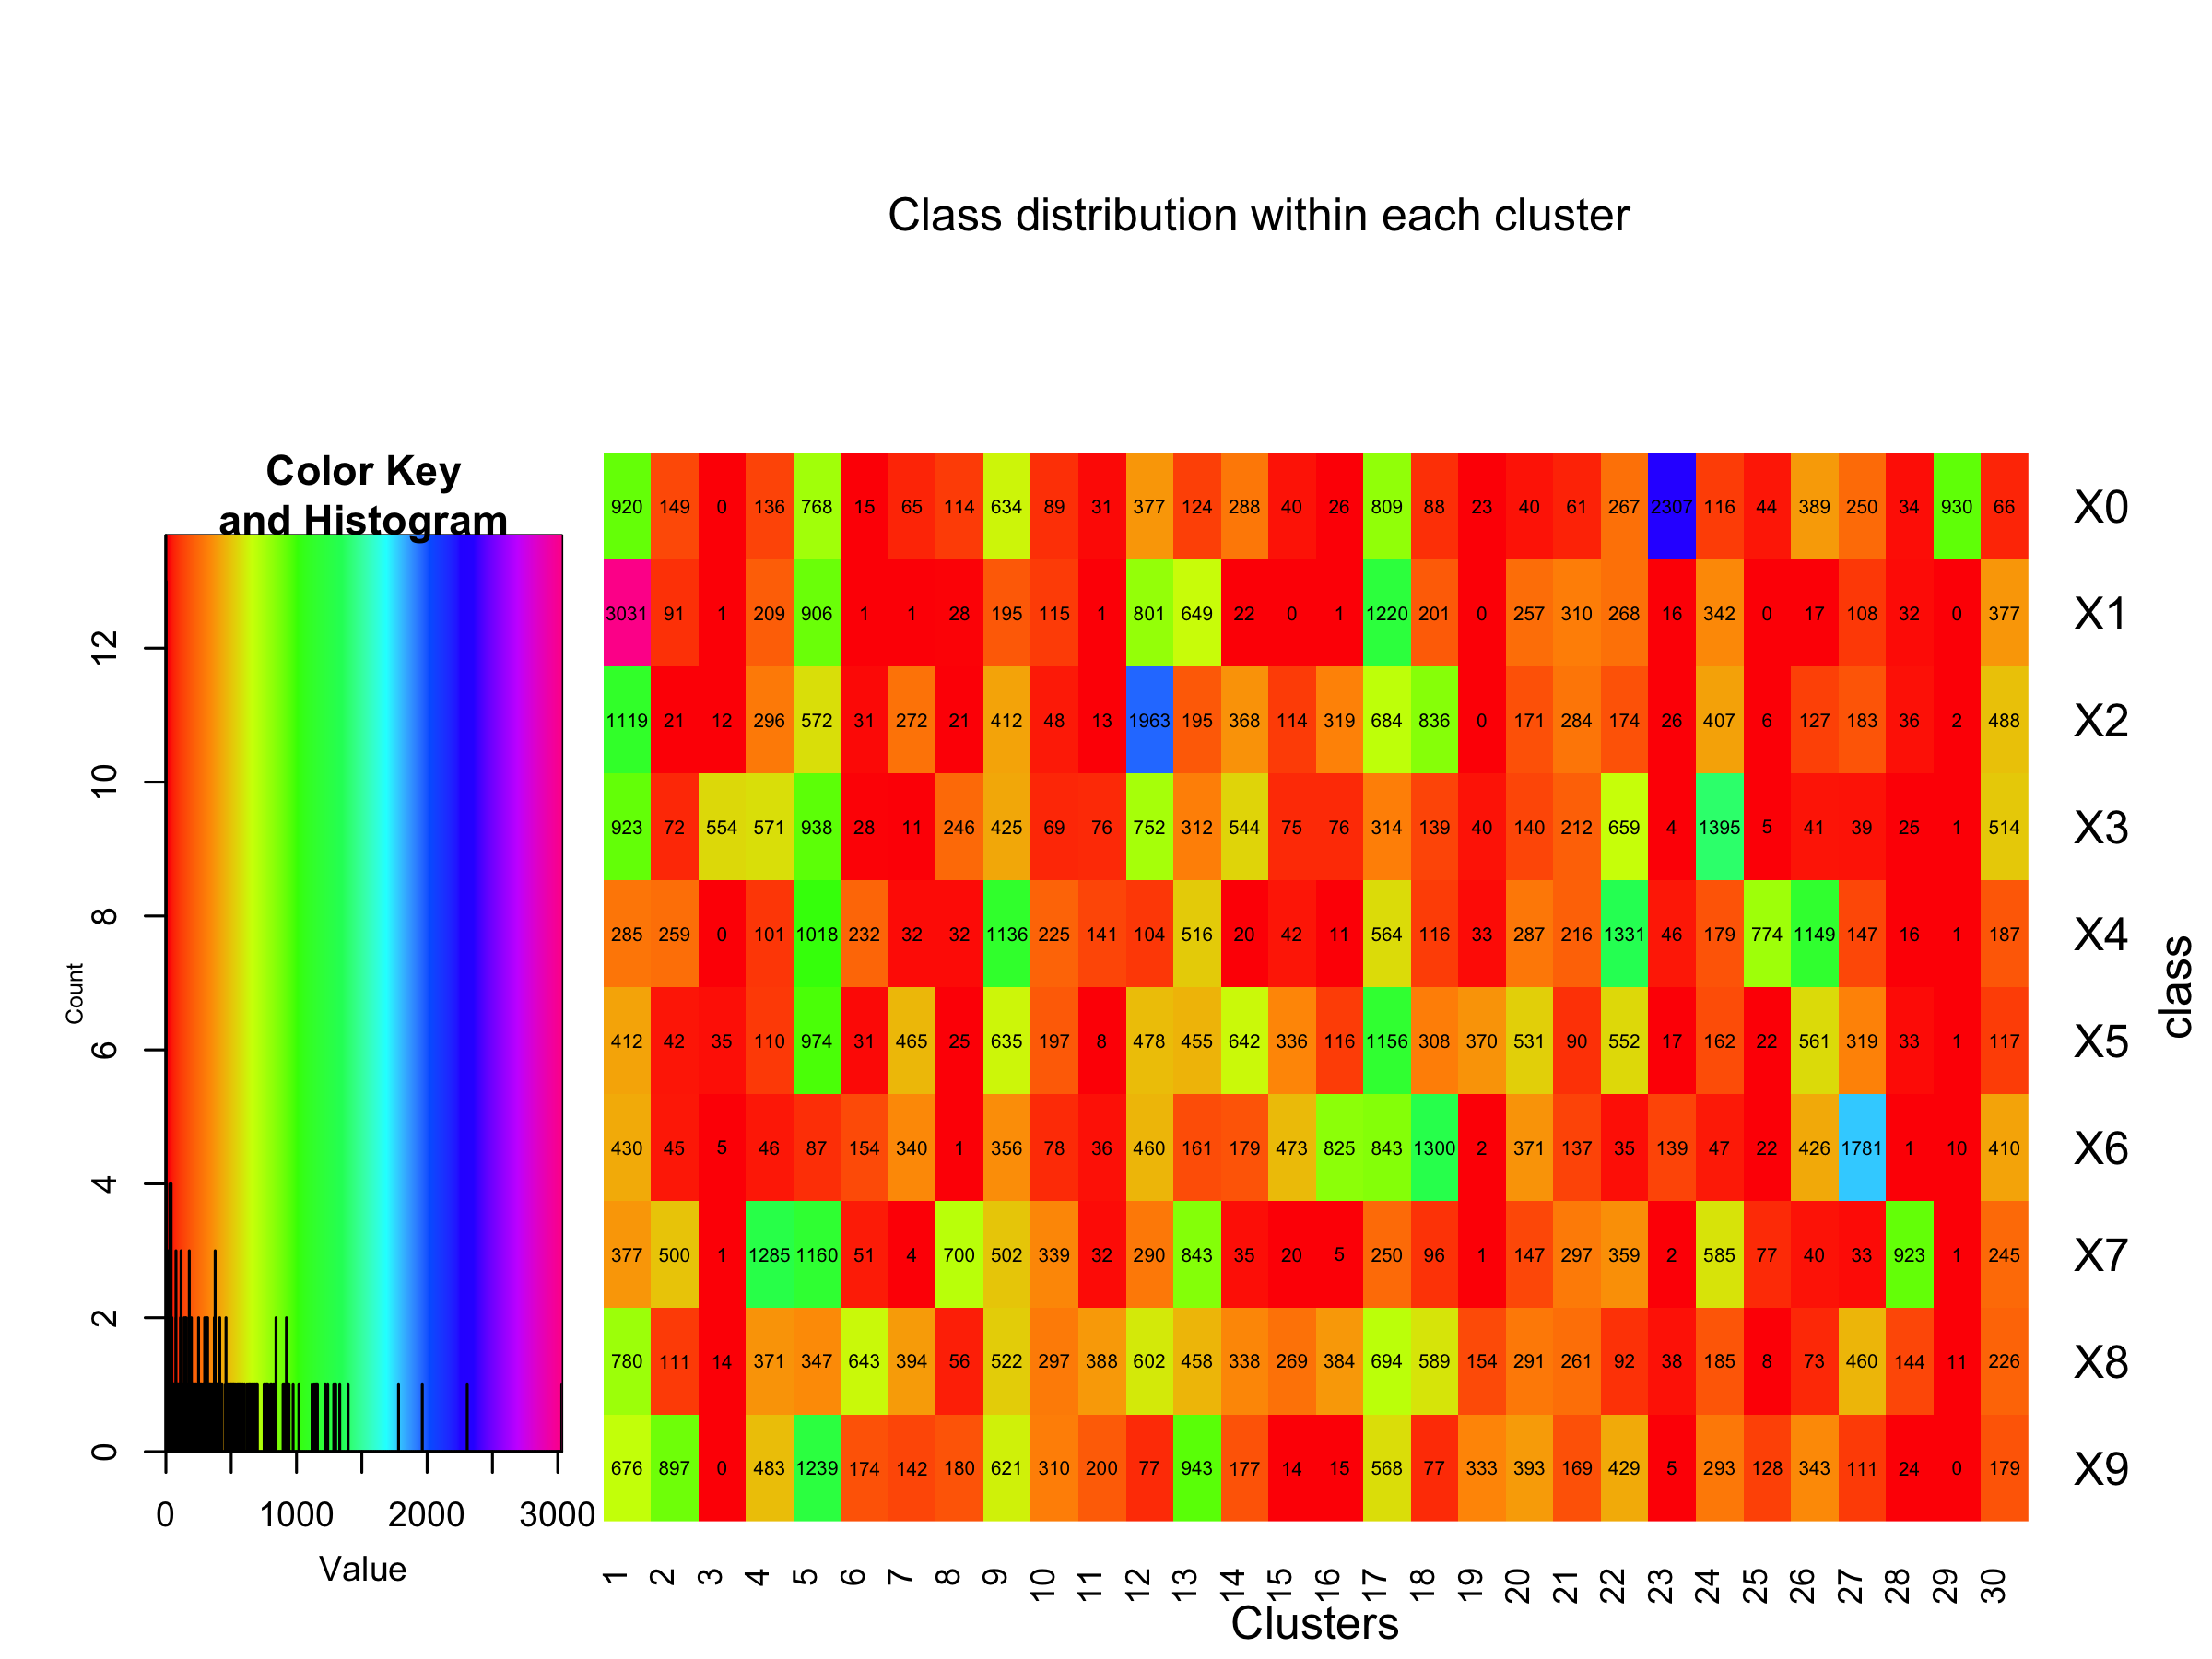
\includegraphics[width = 0.7\textwidth]{heatmap_comple.png}\label{fig:complete}} 

  		\subfloat[Clustering data consiting of digit 0]{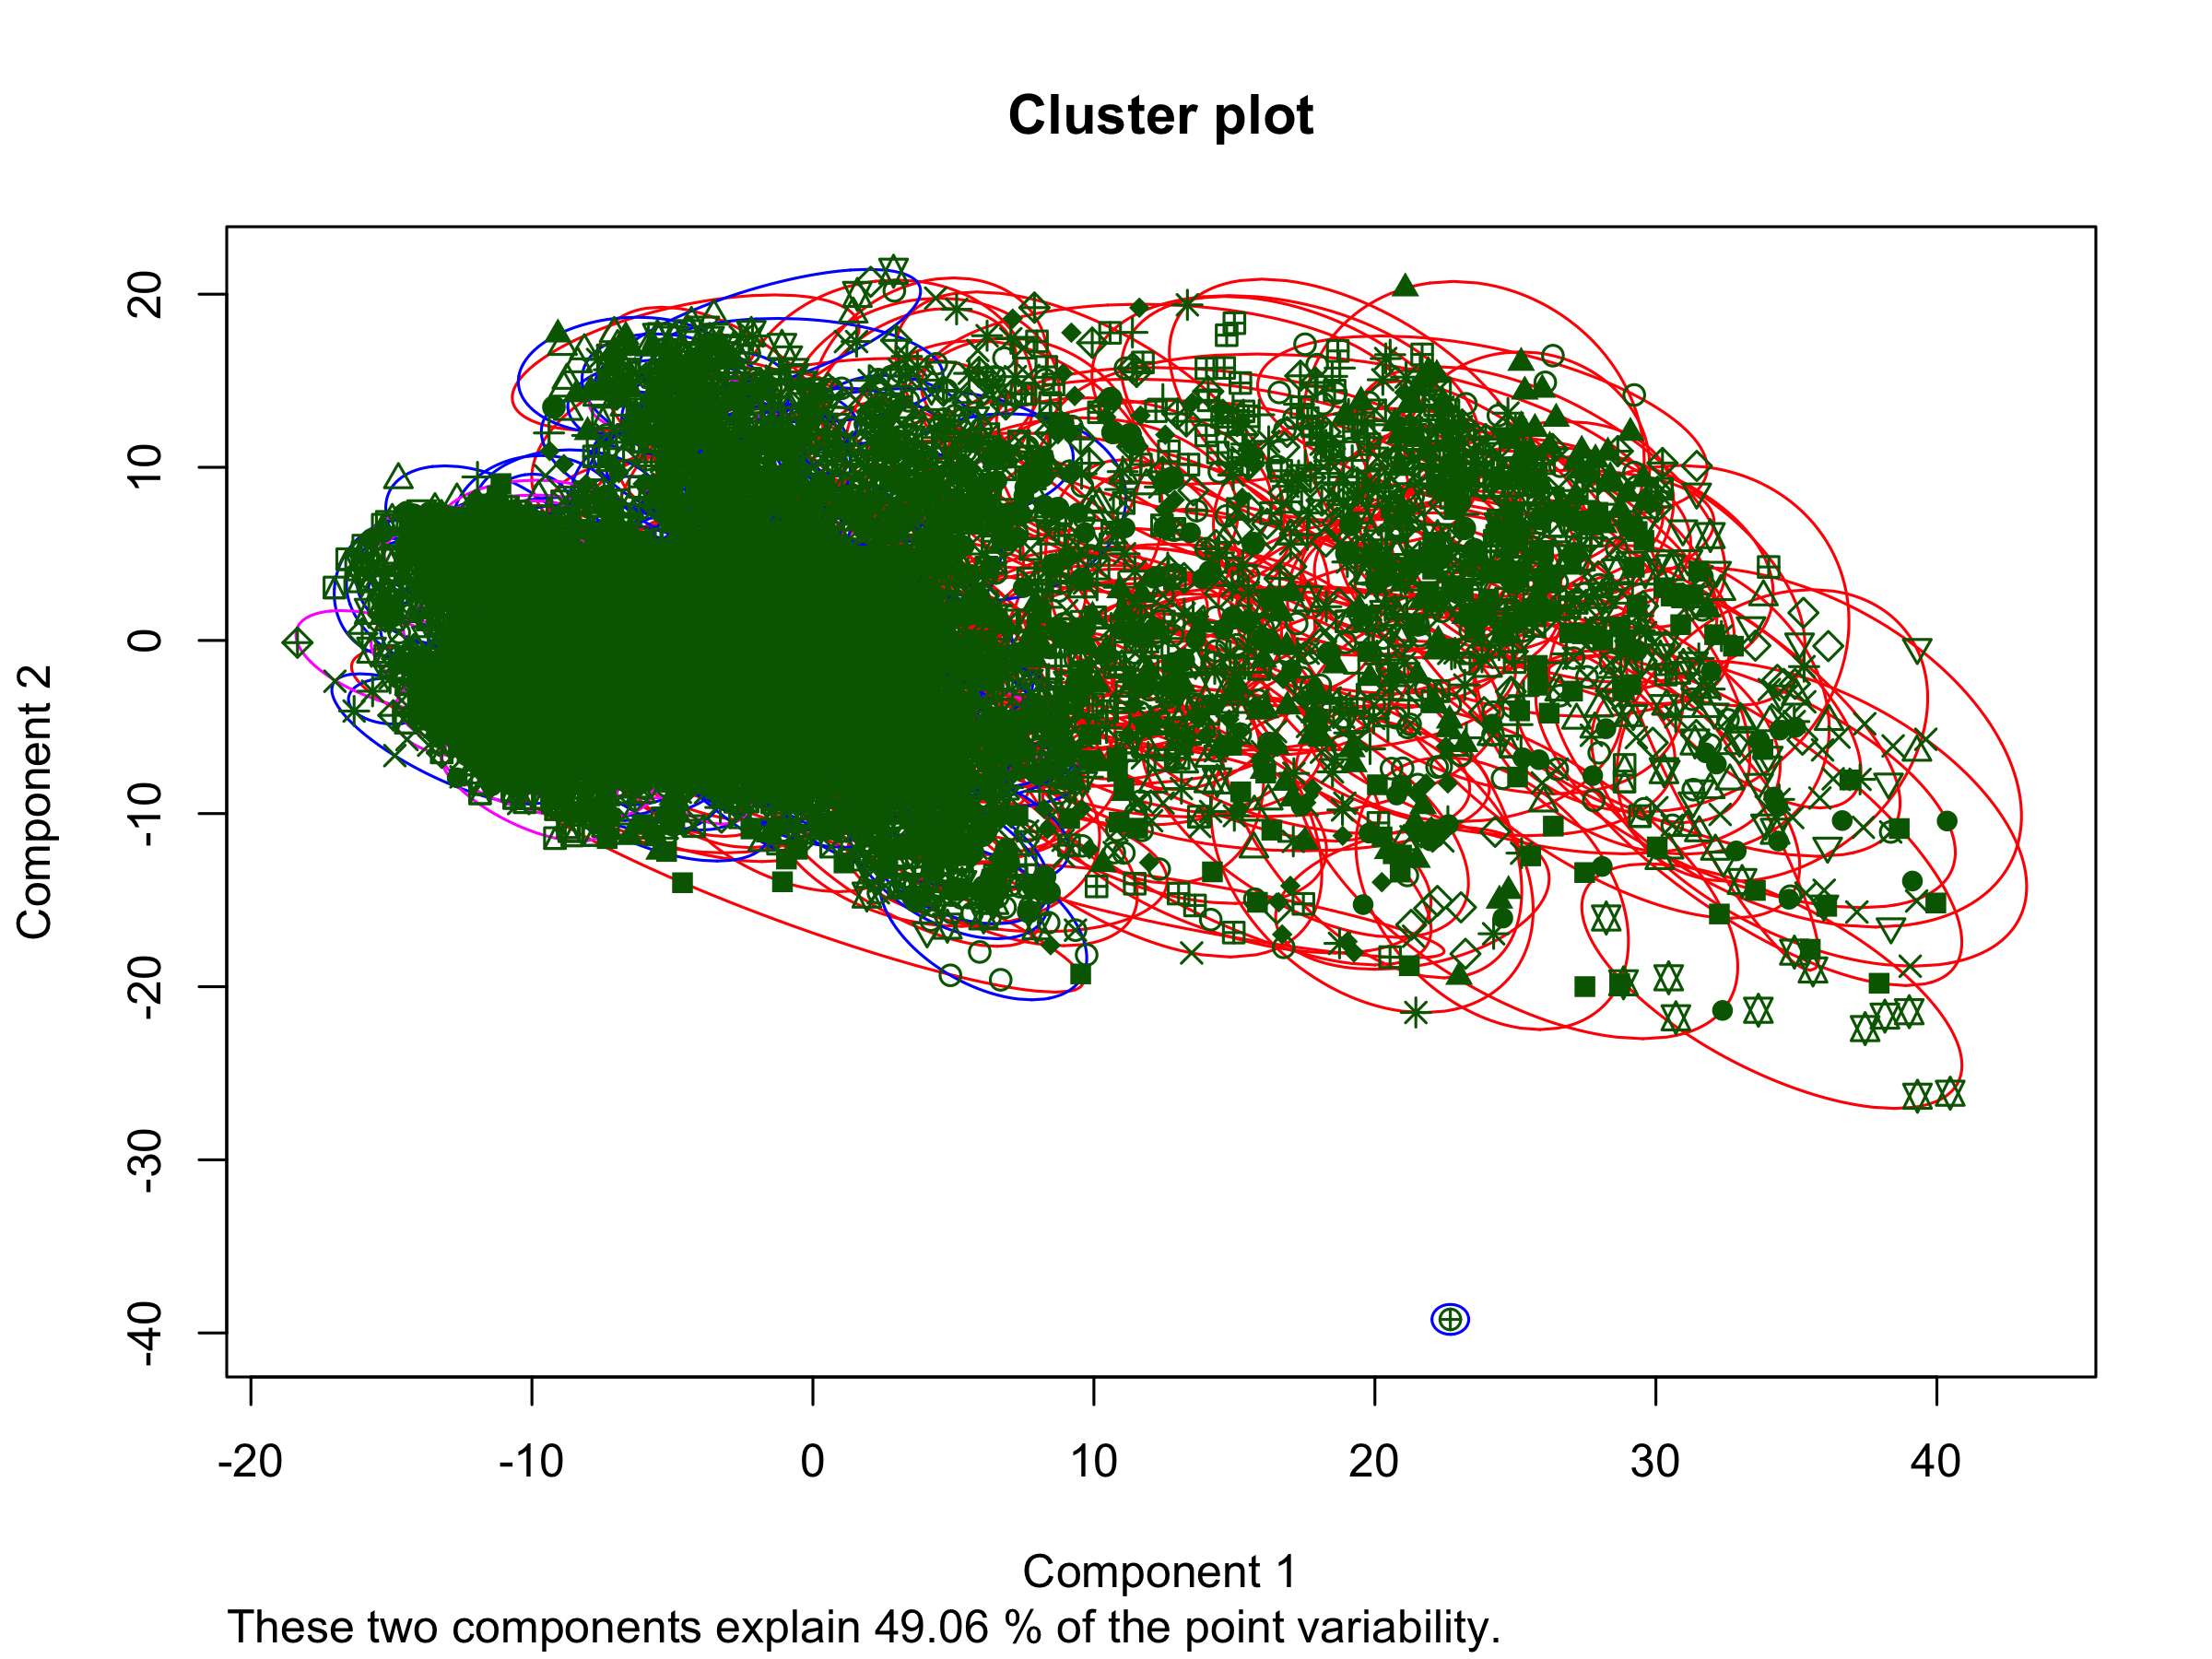
\includegraphics[width = 0.2\textwidth]{clusplot_0.png}\label{fig:0}}\hspace{1em}
%  		
  		\subfloat[Clustering data consiting of digit 1]{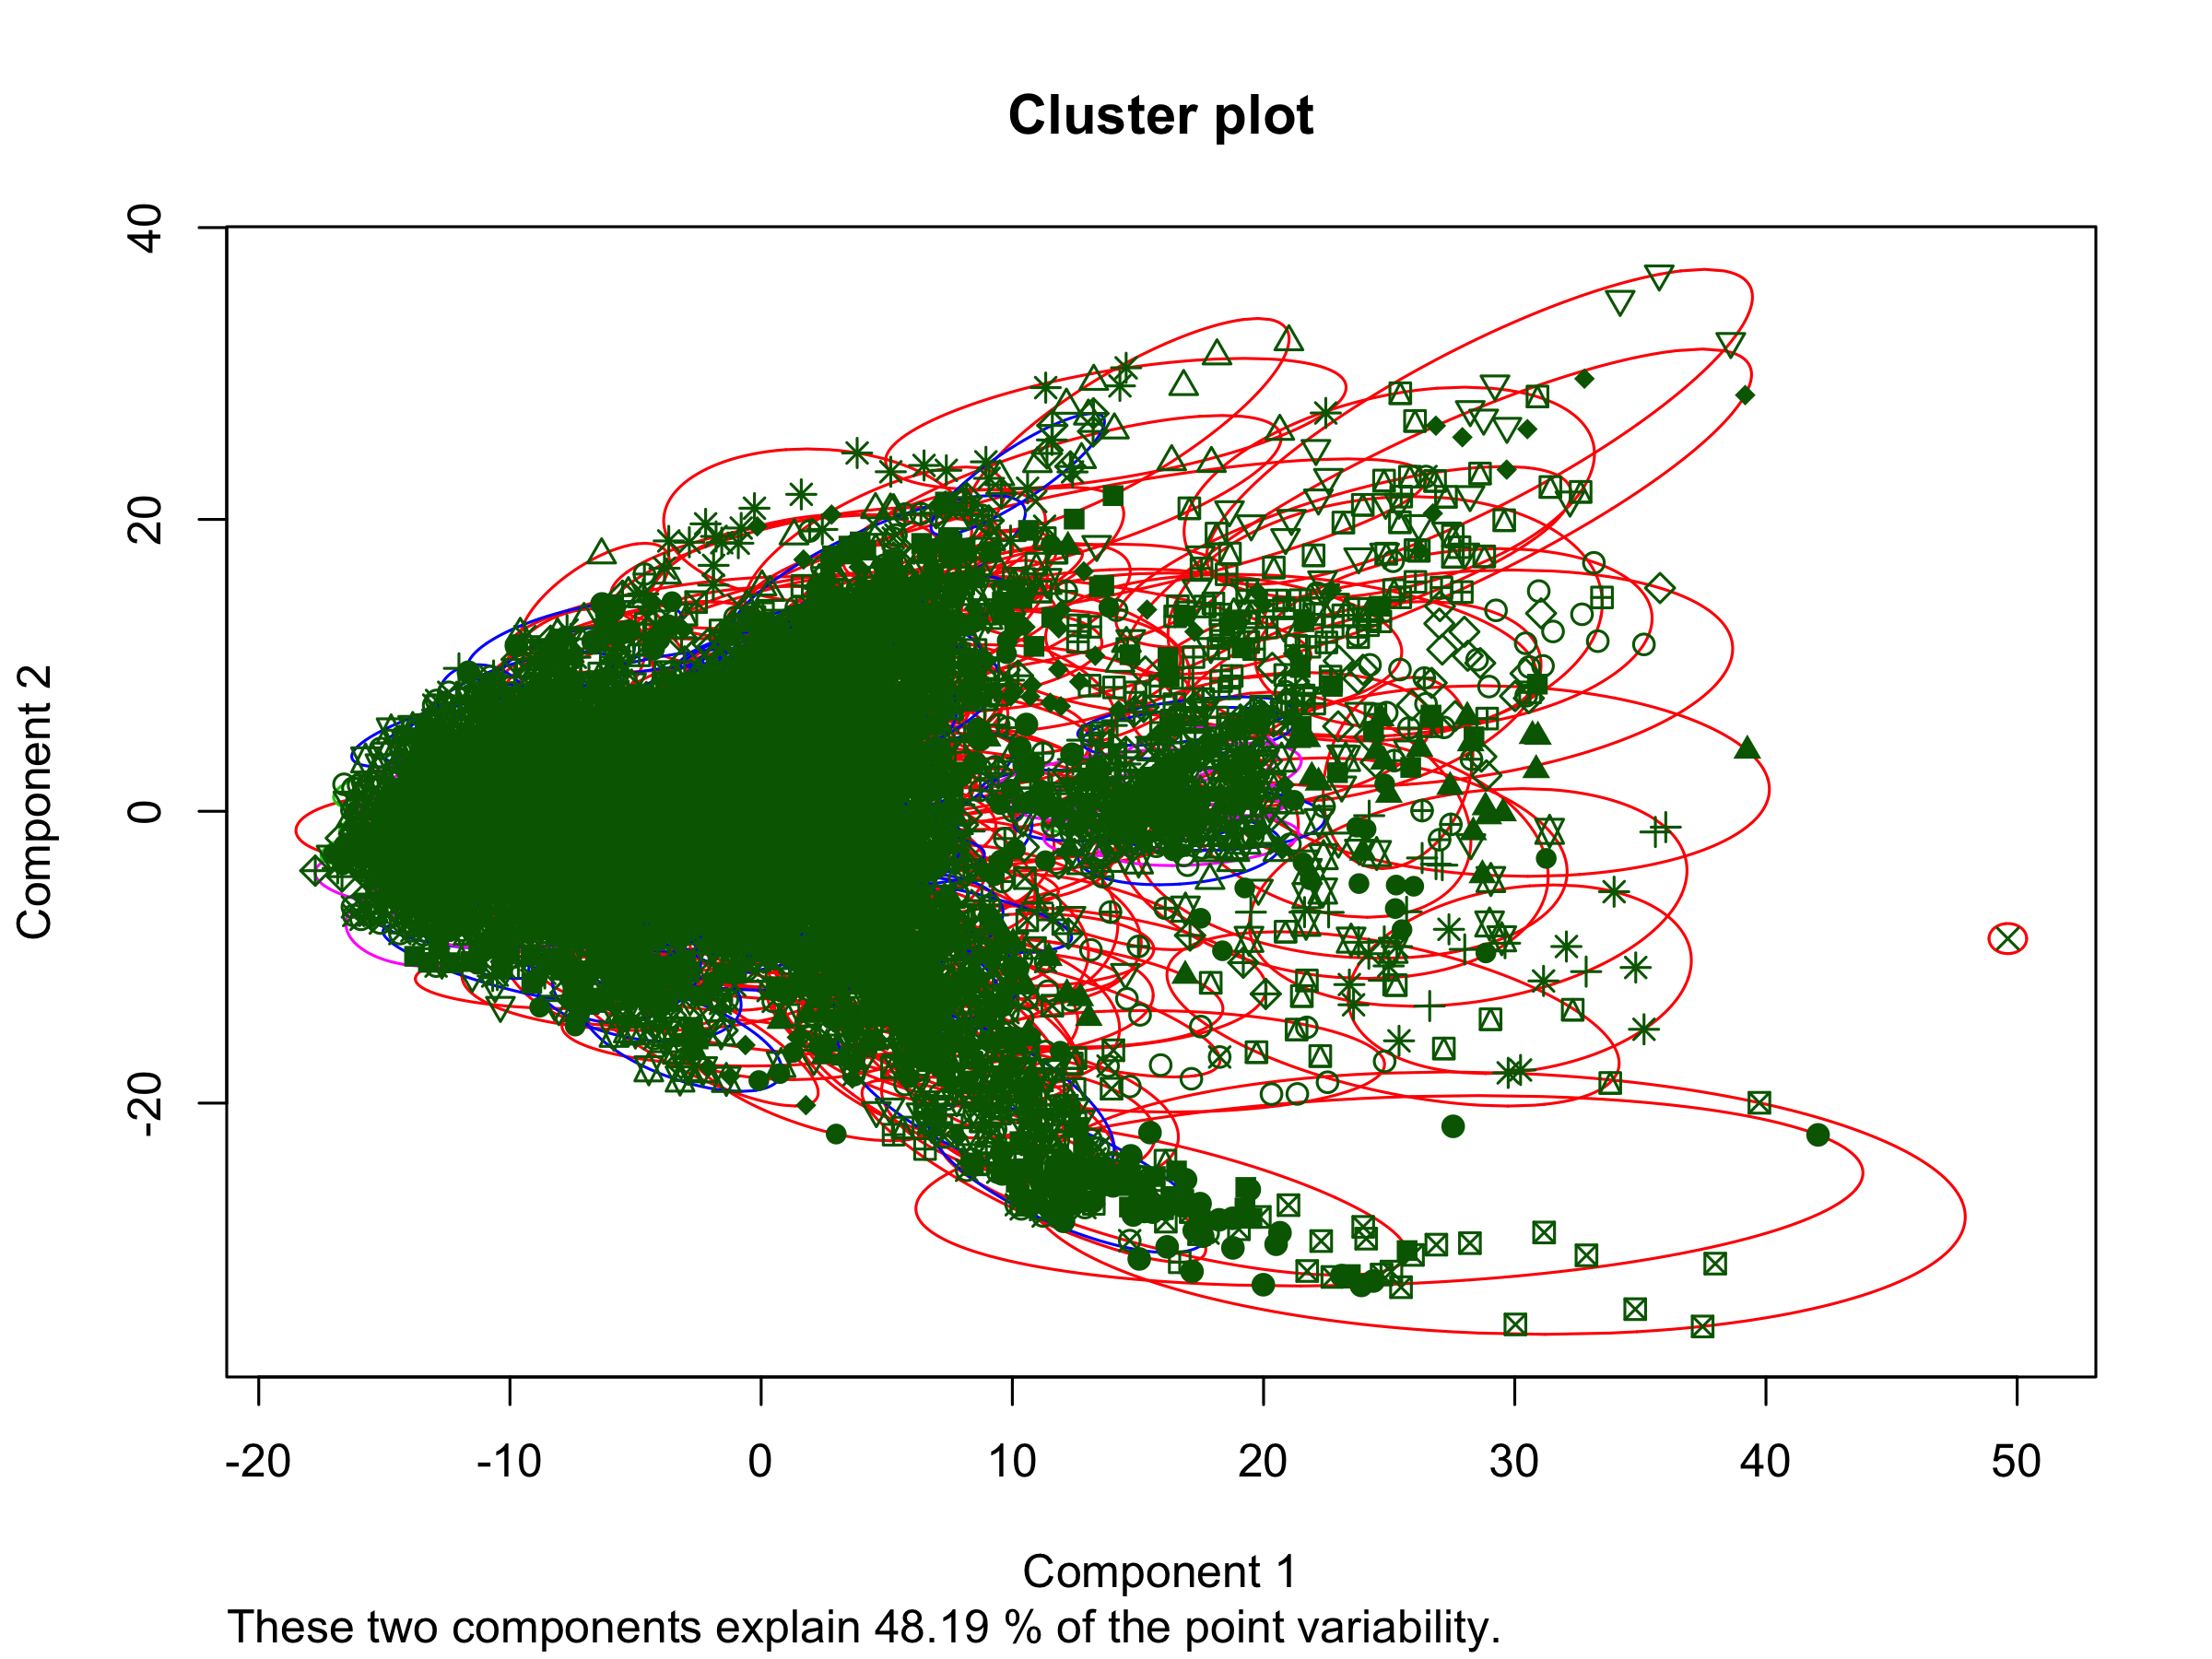
\includegraphics[width = 0.2\textwidth]{clusplot_1.png}\label{fig:1}}
%
  		\subfloat[Clustering data consiting of digit 2]{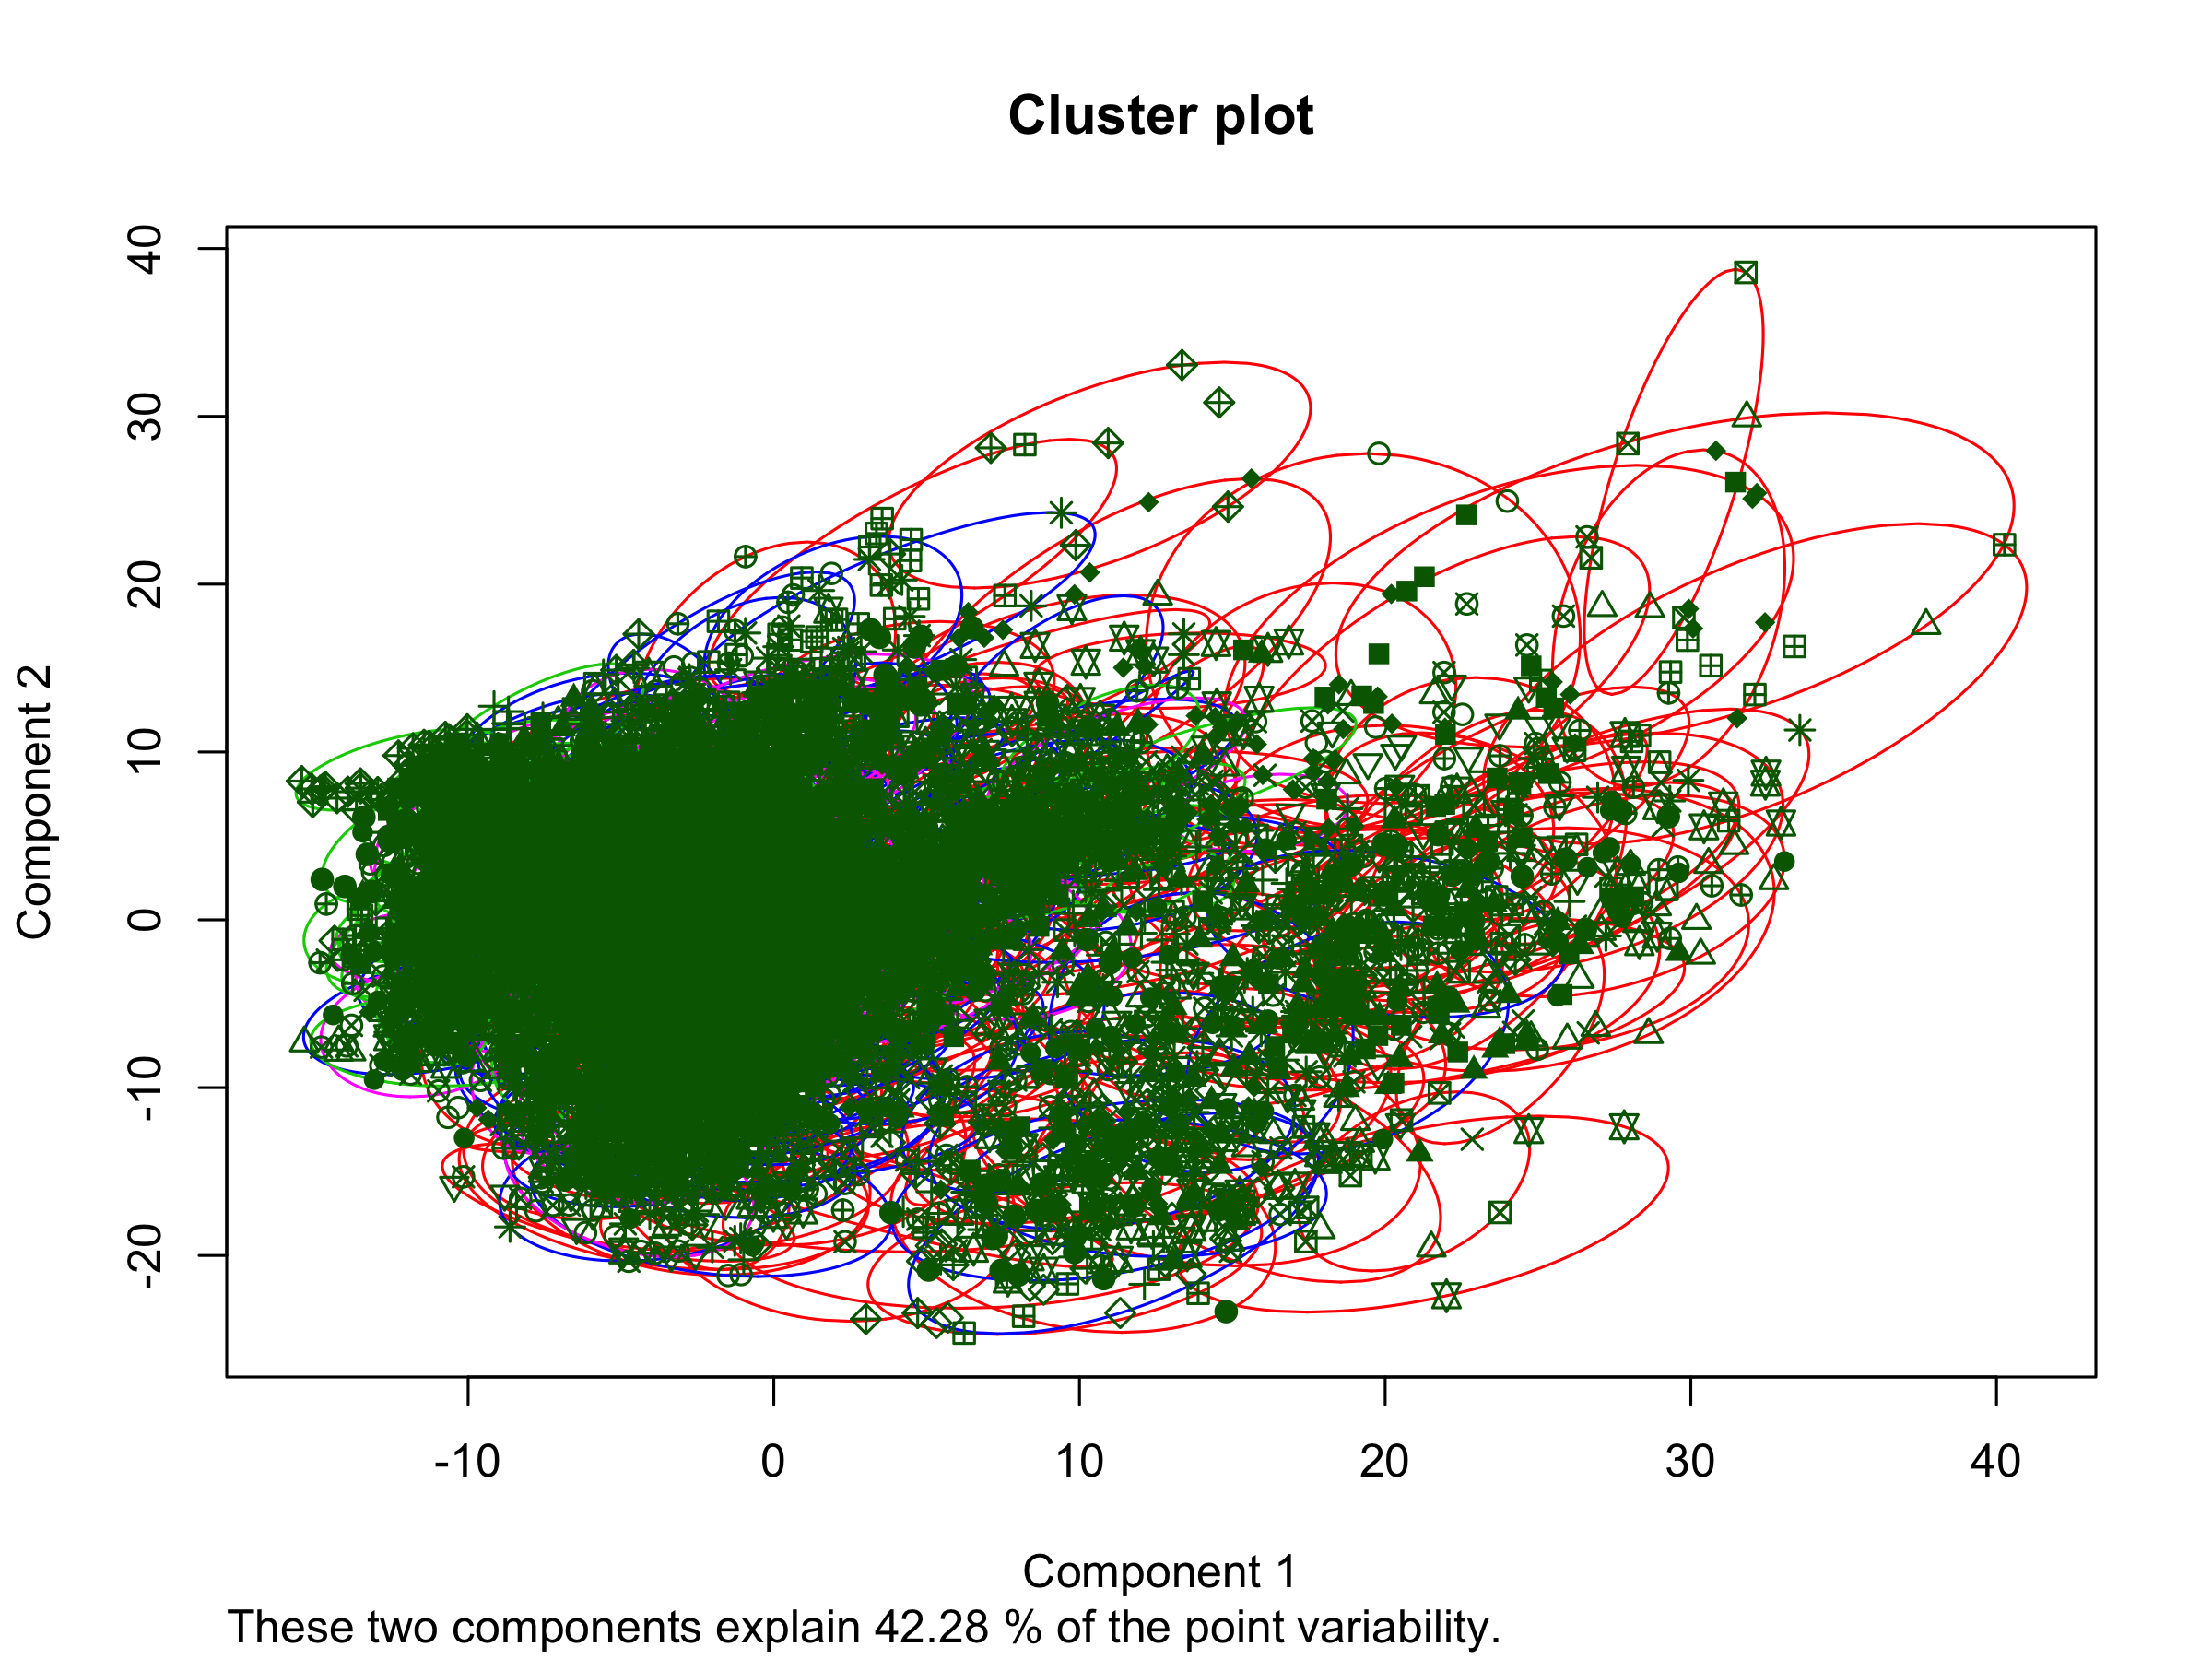
\includegraphics[width = 0.2\textwidth]{clusplot_2.png}\label{fig:2}}
%  		
  		\subfloat[Clustering data consiting of digit 3]{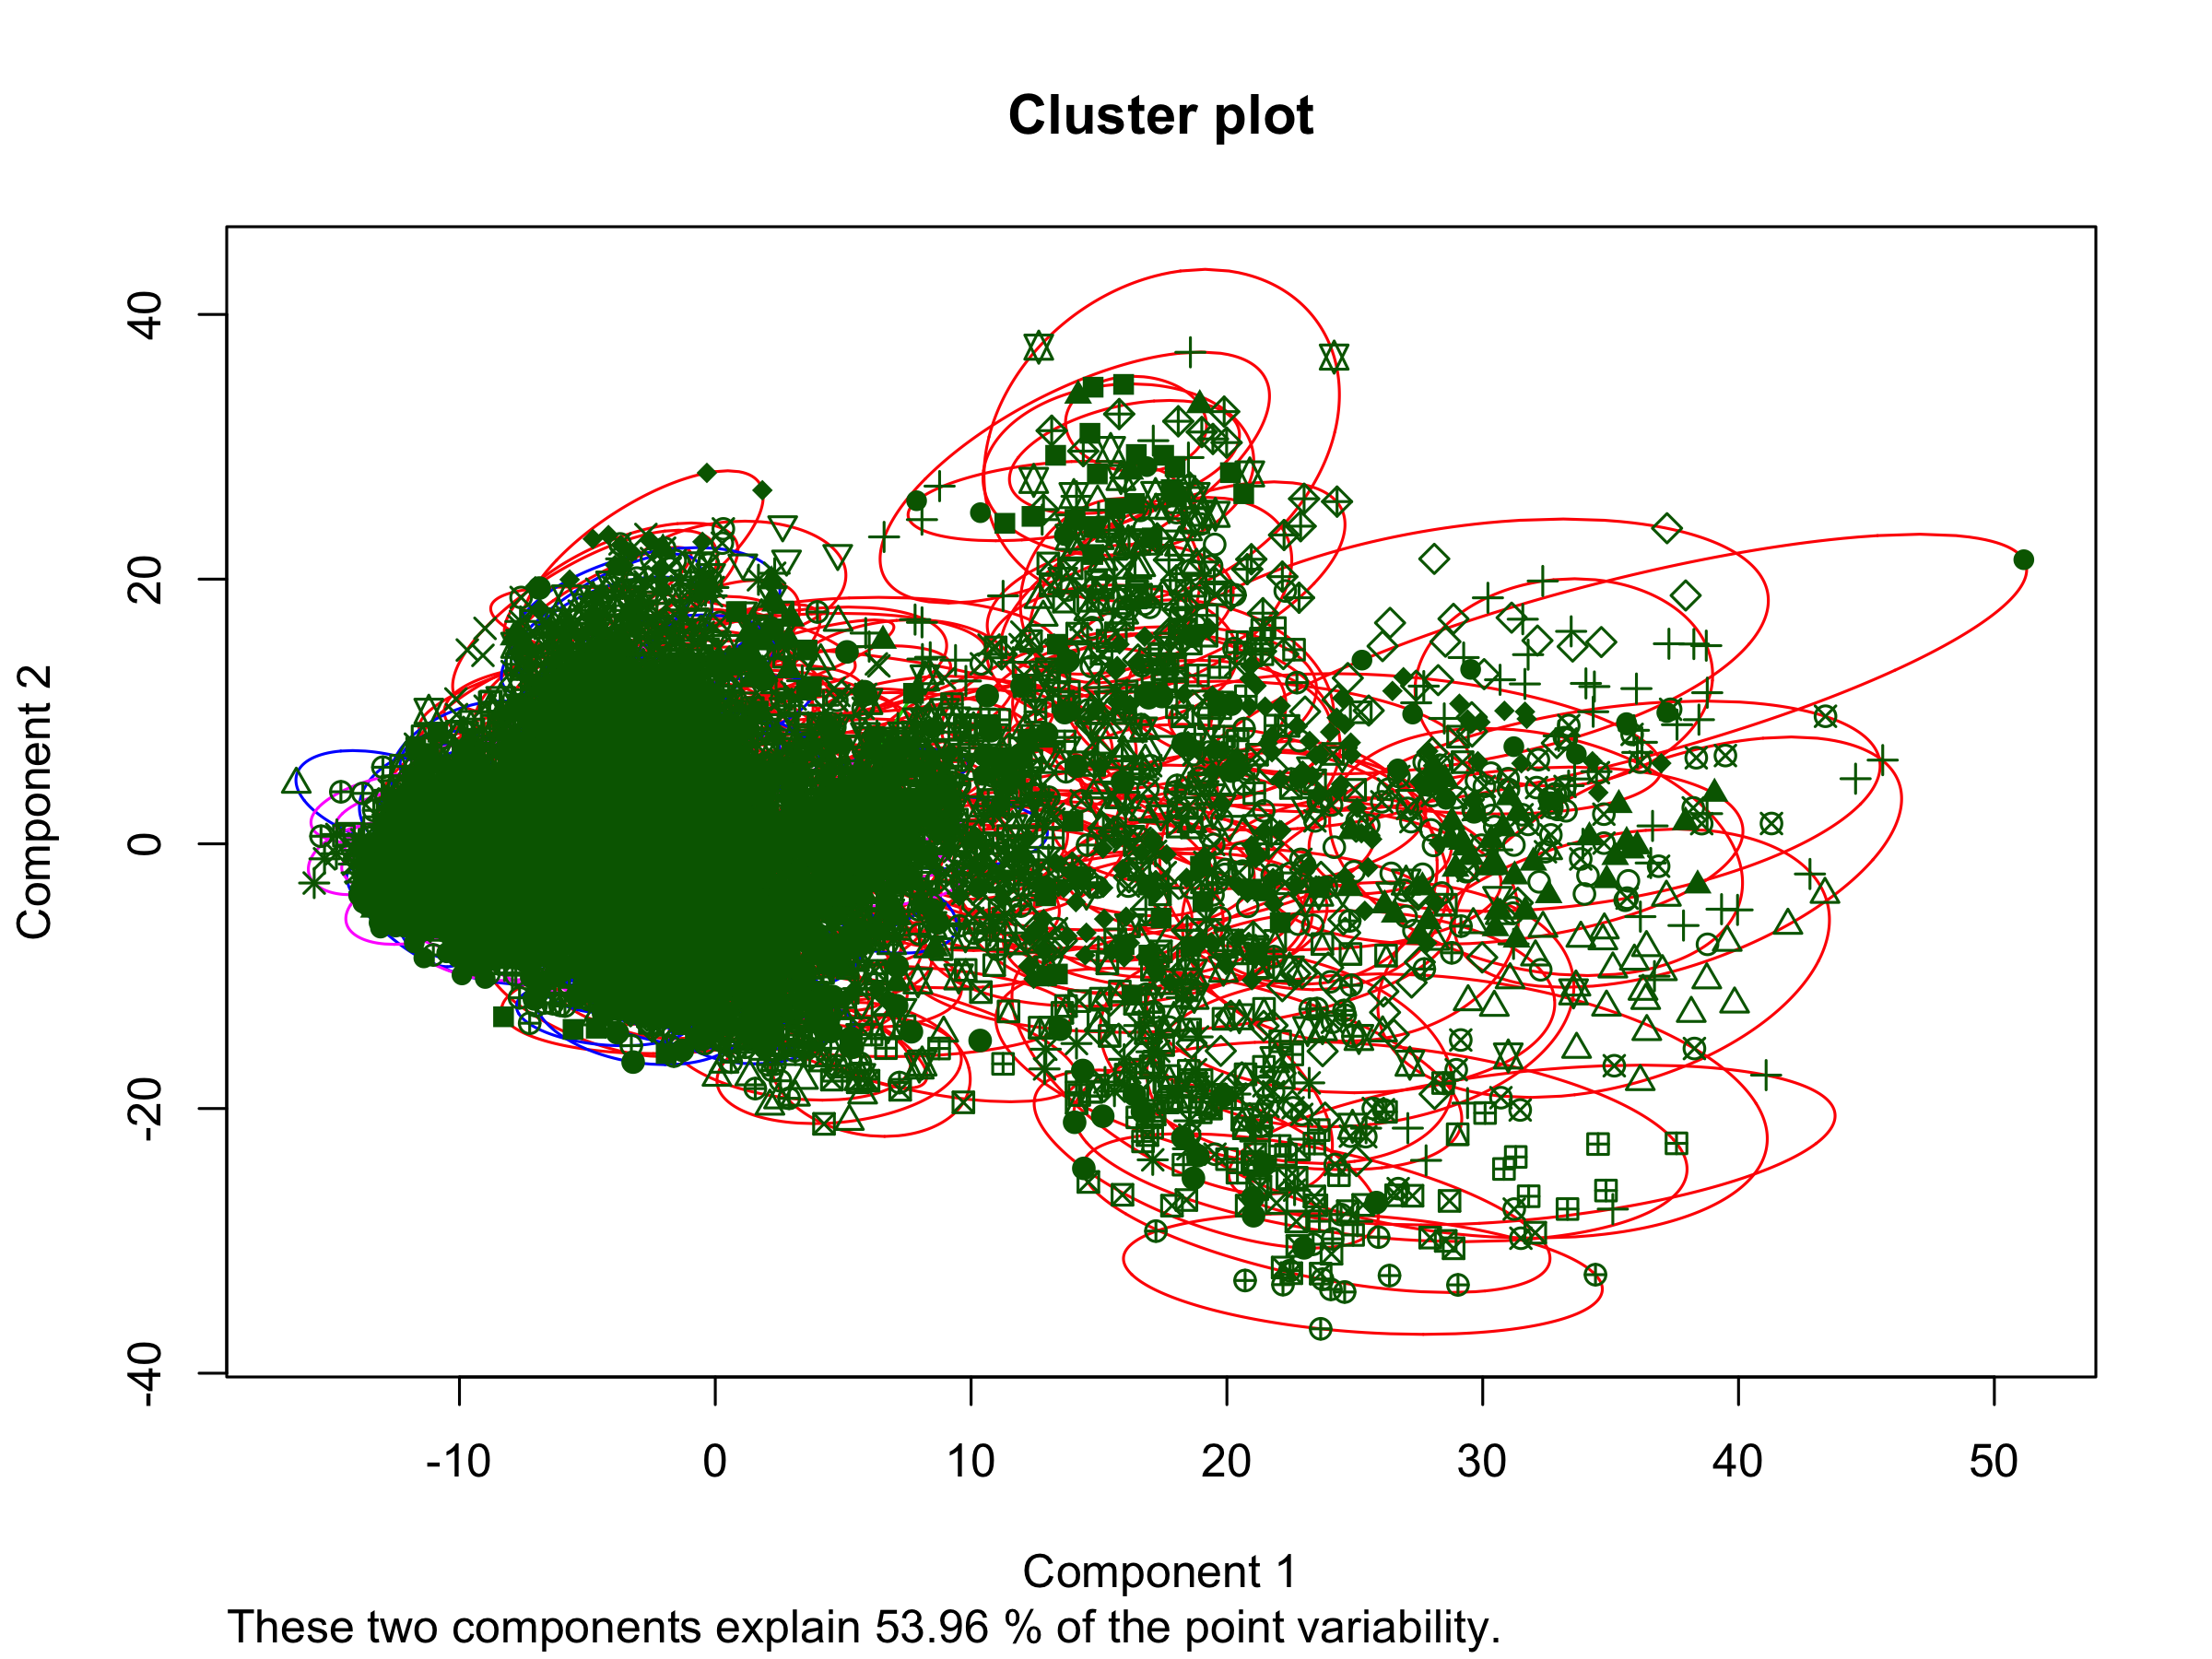
\includegraphics[width = 0.2\textwidth]{clusplot_3.png}\label{fig:3}}\hspace{1em}
%  		
%  		
  		\subfloat[Clustering data consiting of digit 4]{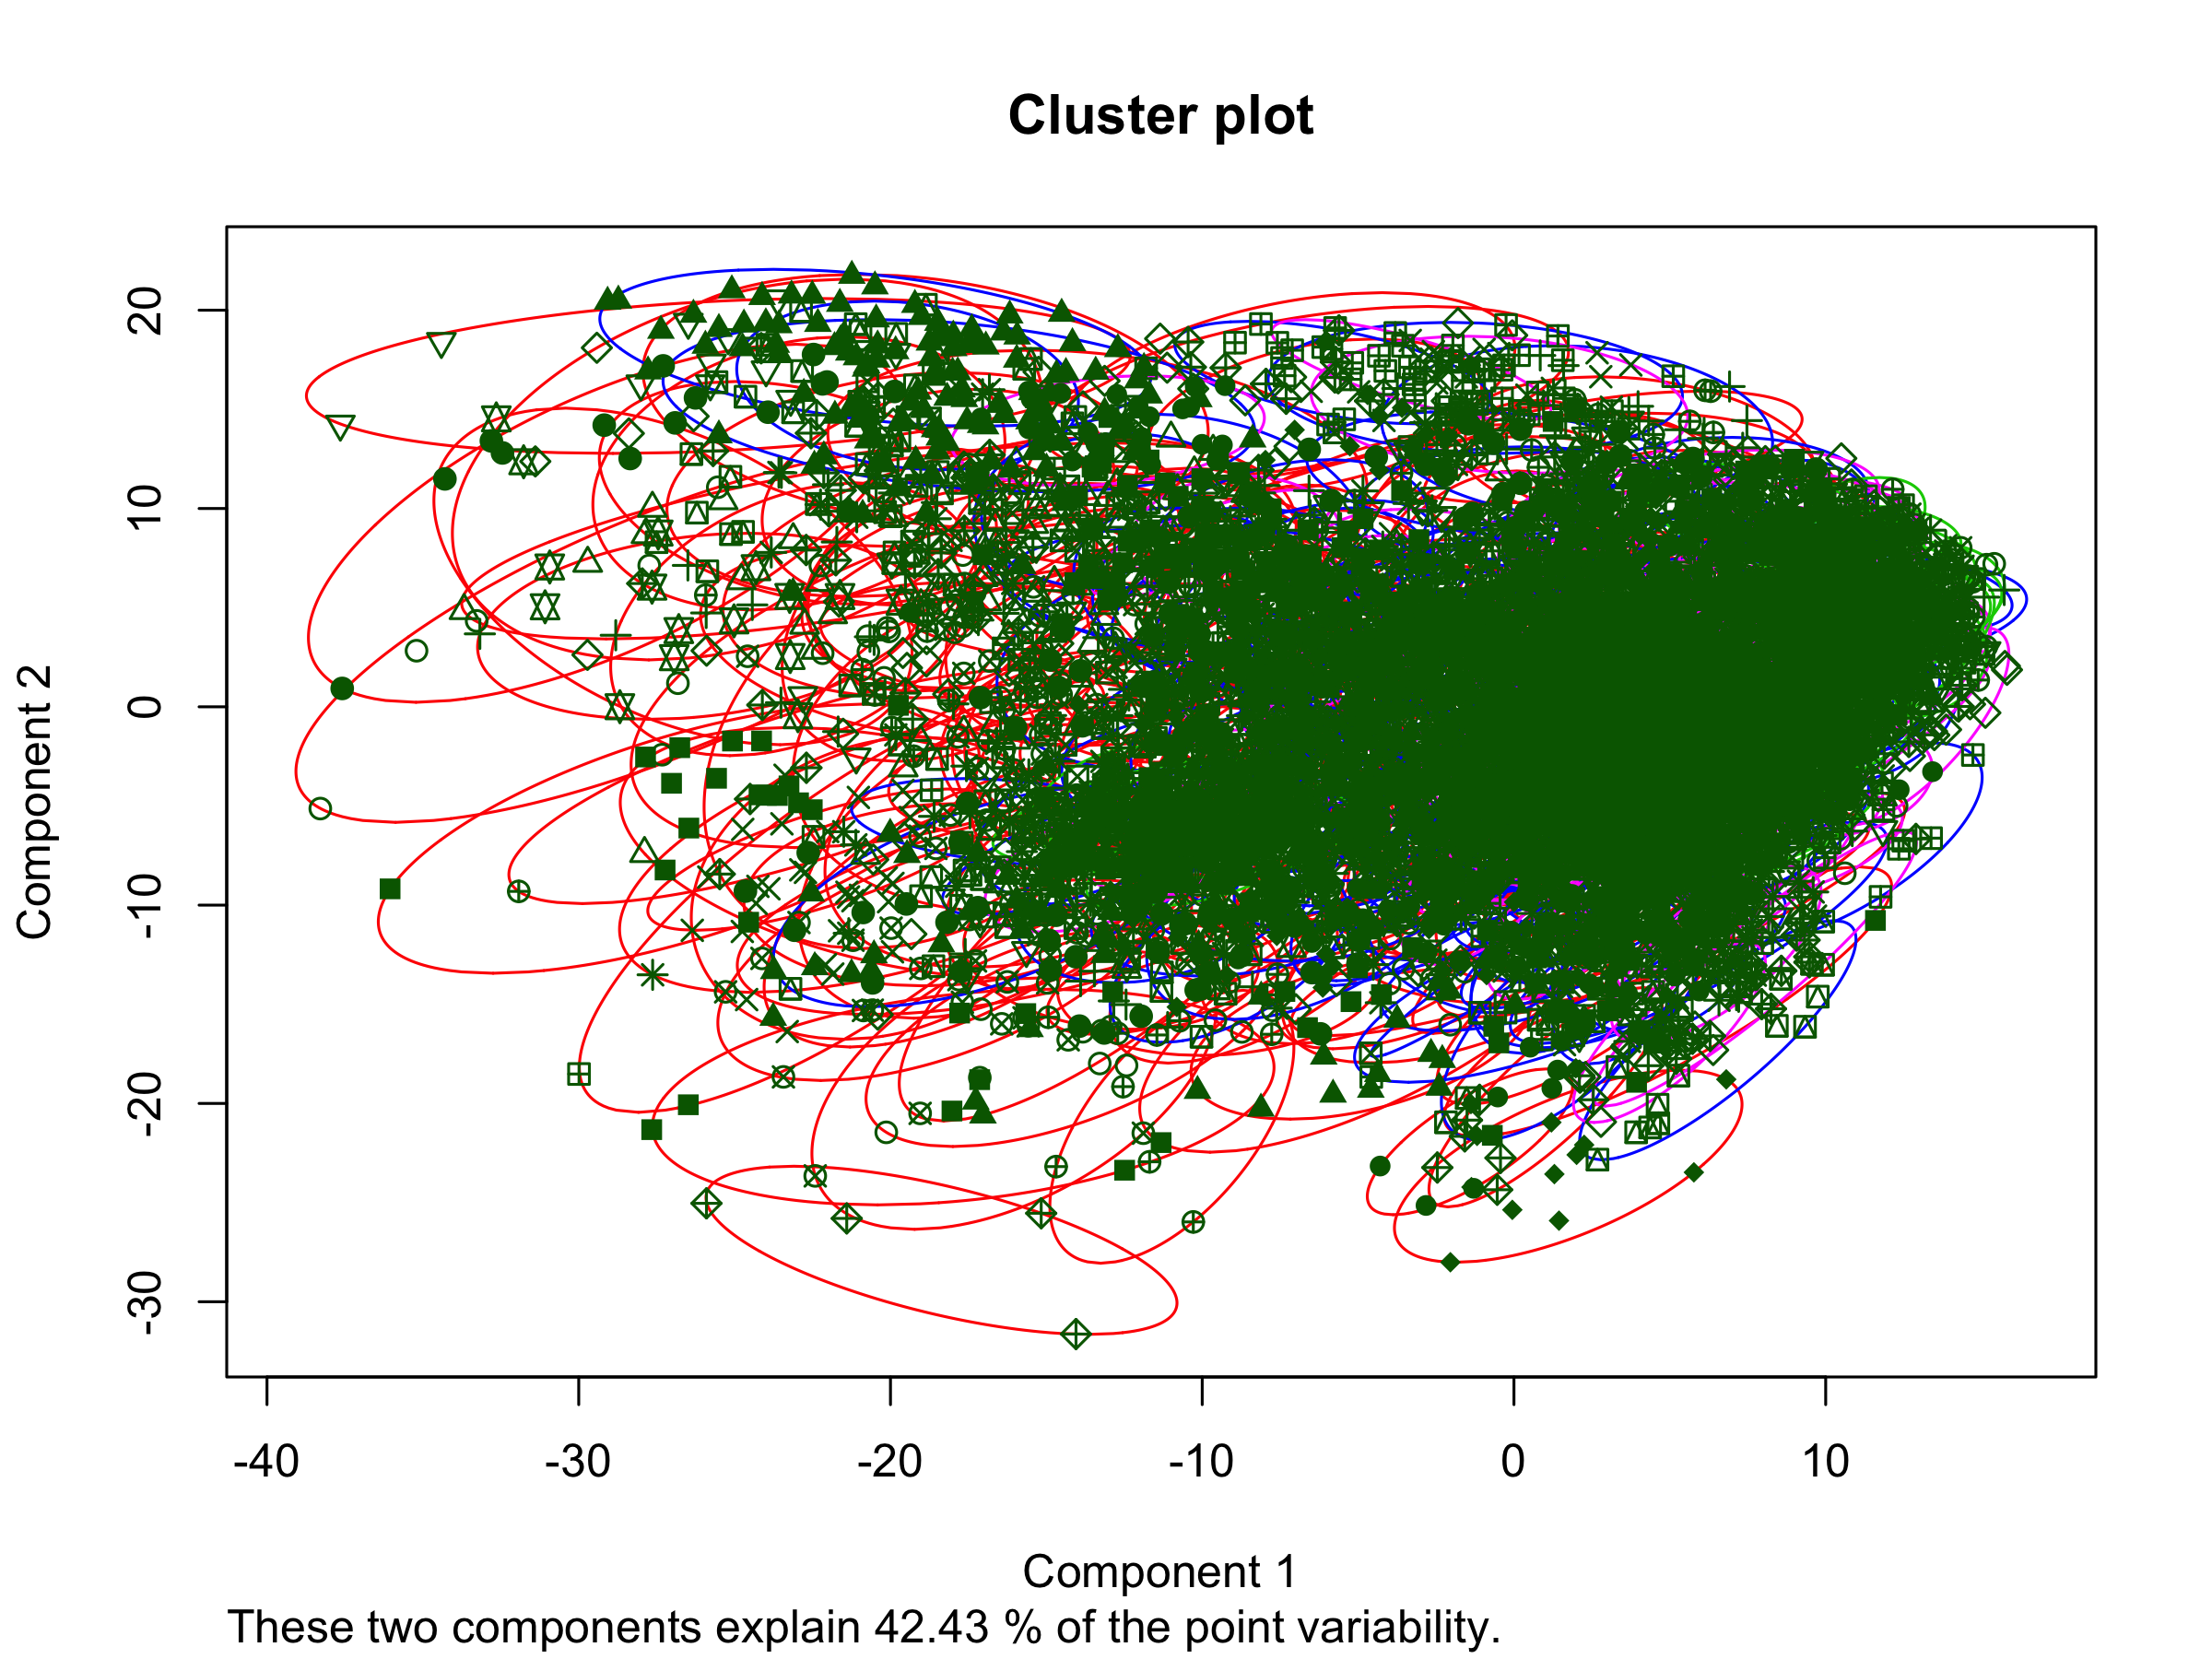
\includegraphics[width = 0.2\textwidth]{clusplot_4.png}\label{fig:4}}
%  		
  		\subfloat[Clustering data consiting of digit 5]{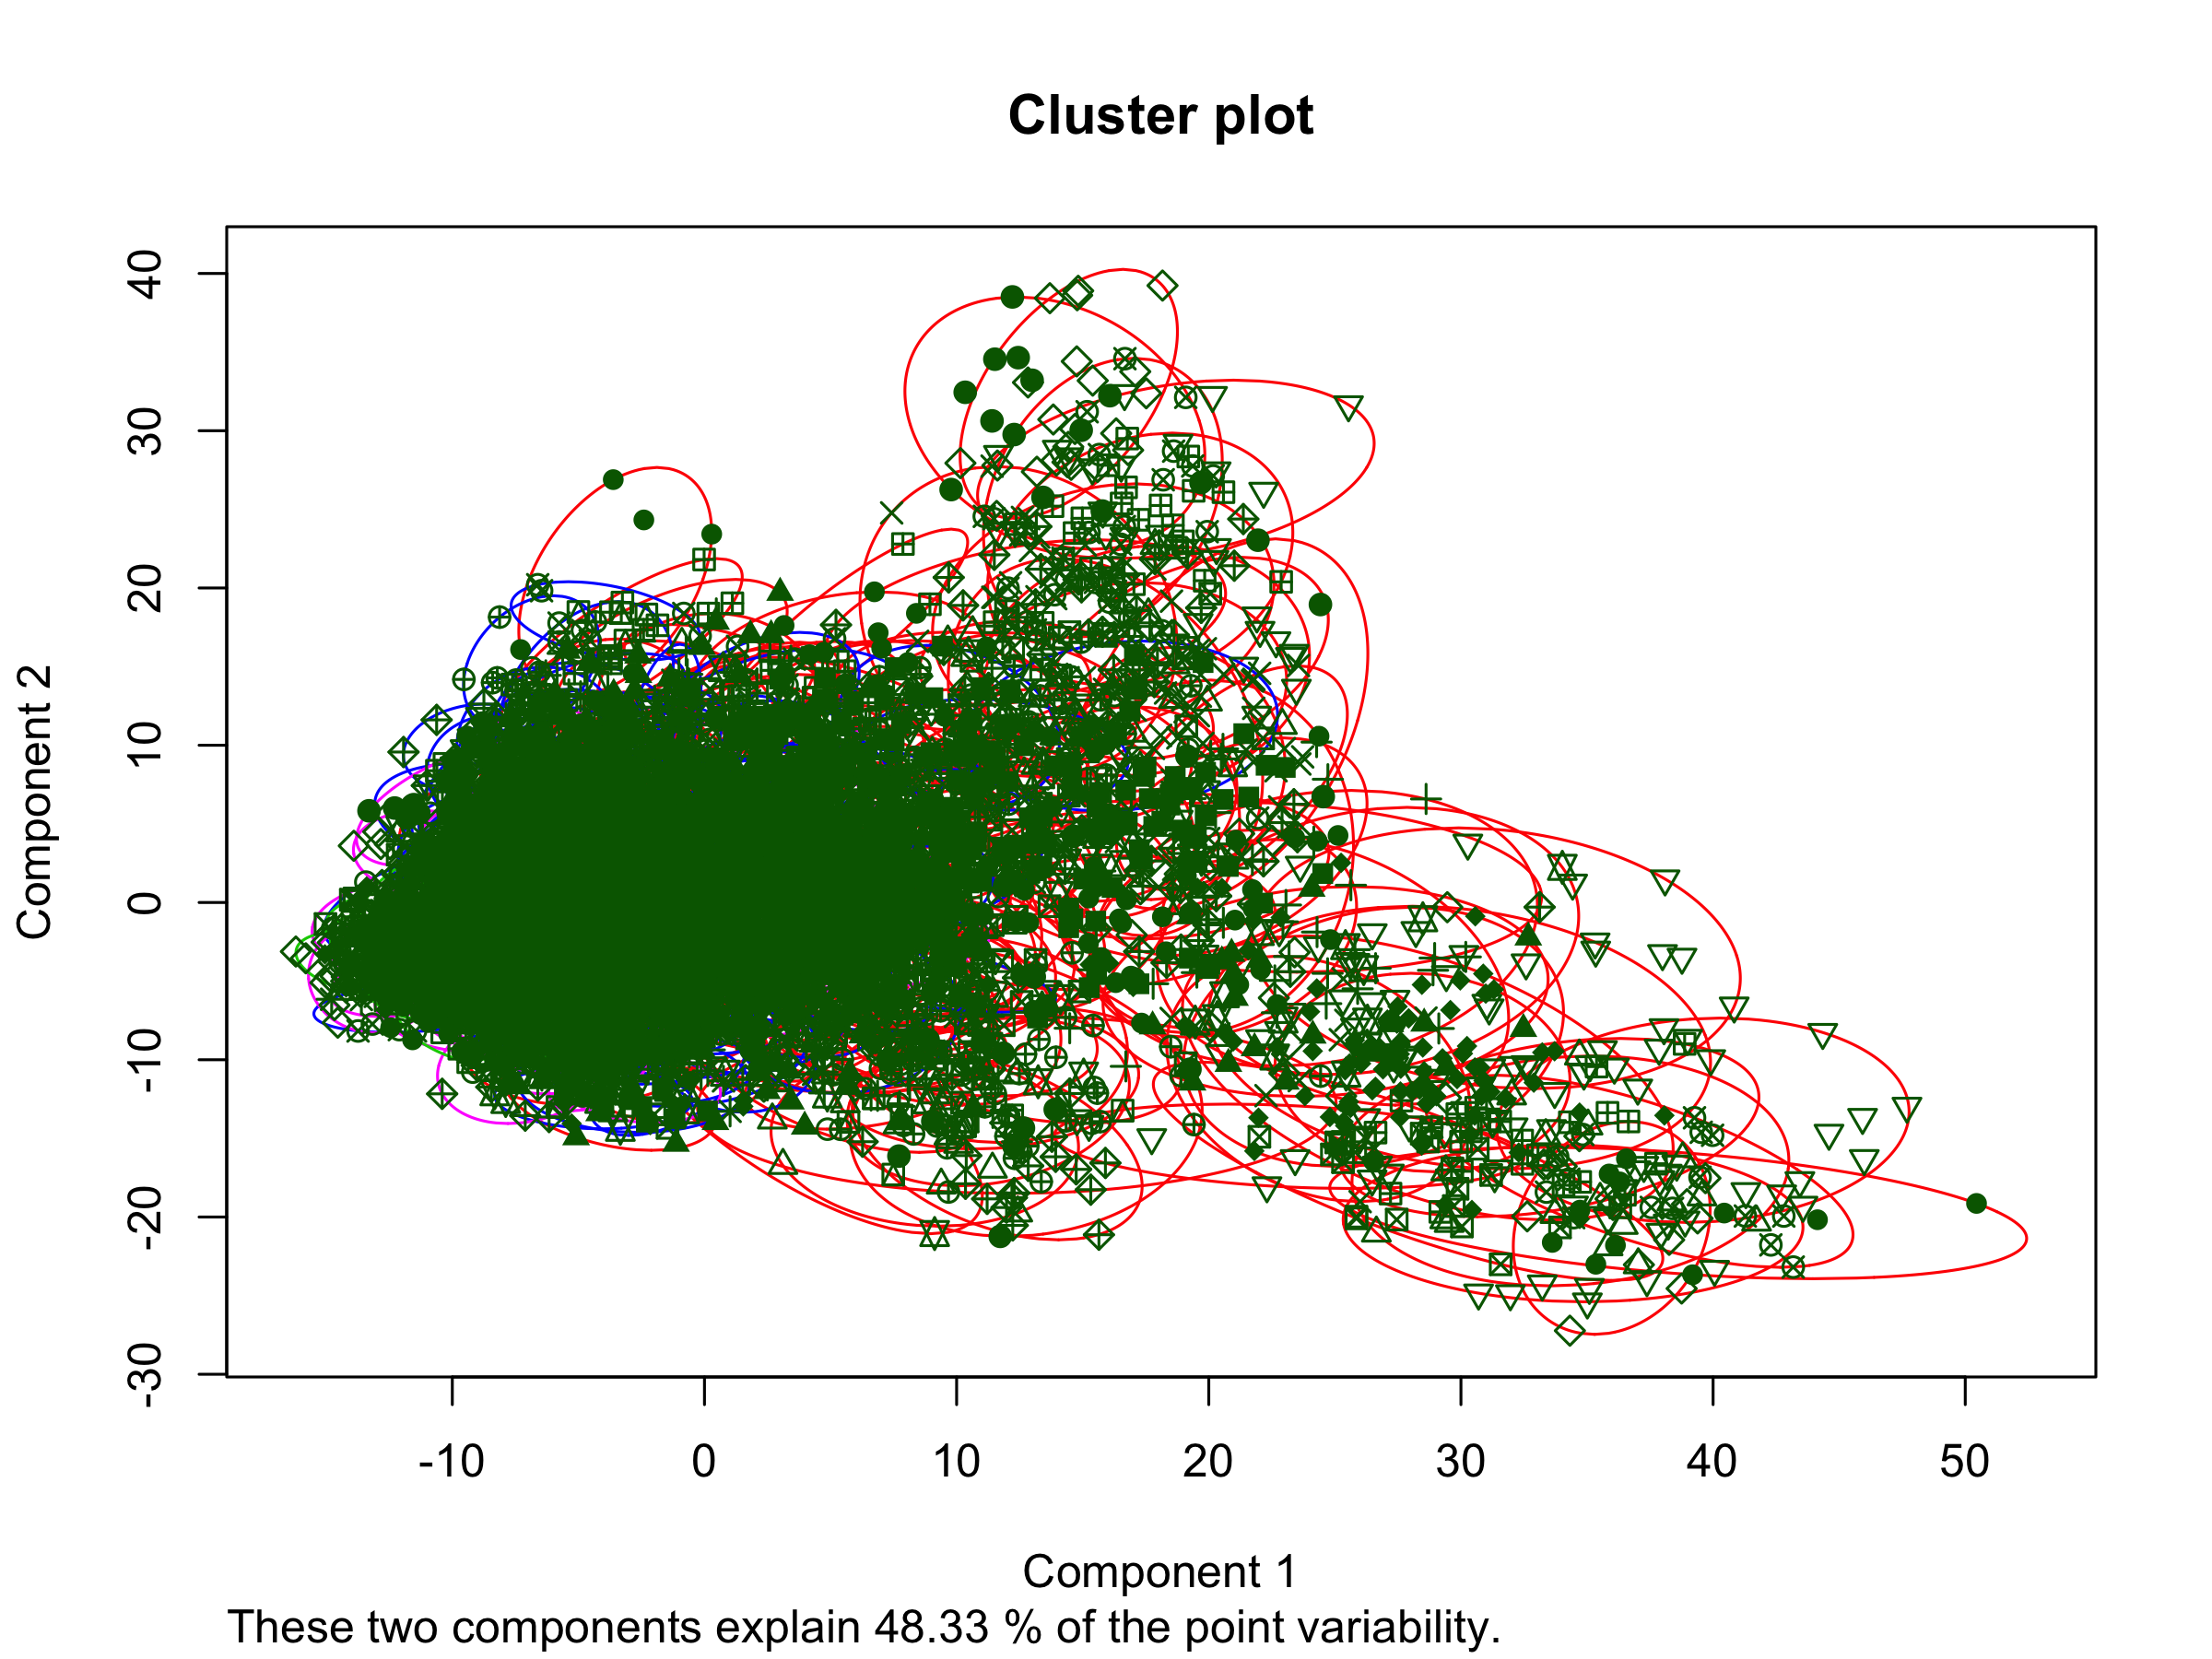
\includegraphics[width = 0.2\textwidth]{clusplot_5.png}\label{fig:5}}
%  			
%  			
 		\subfloat[Clustering data consiting of digit 6]{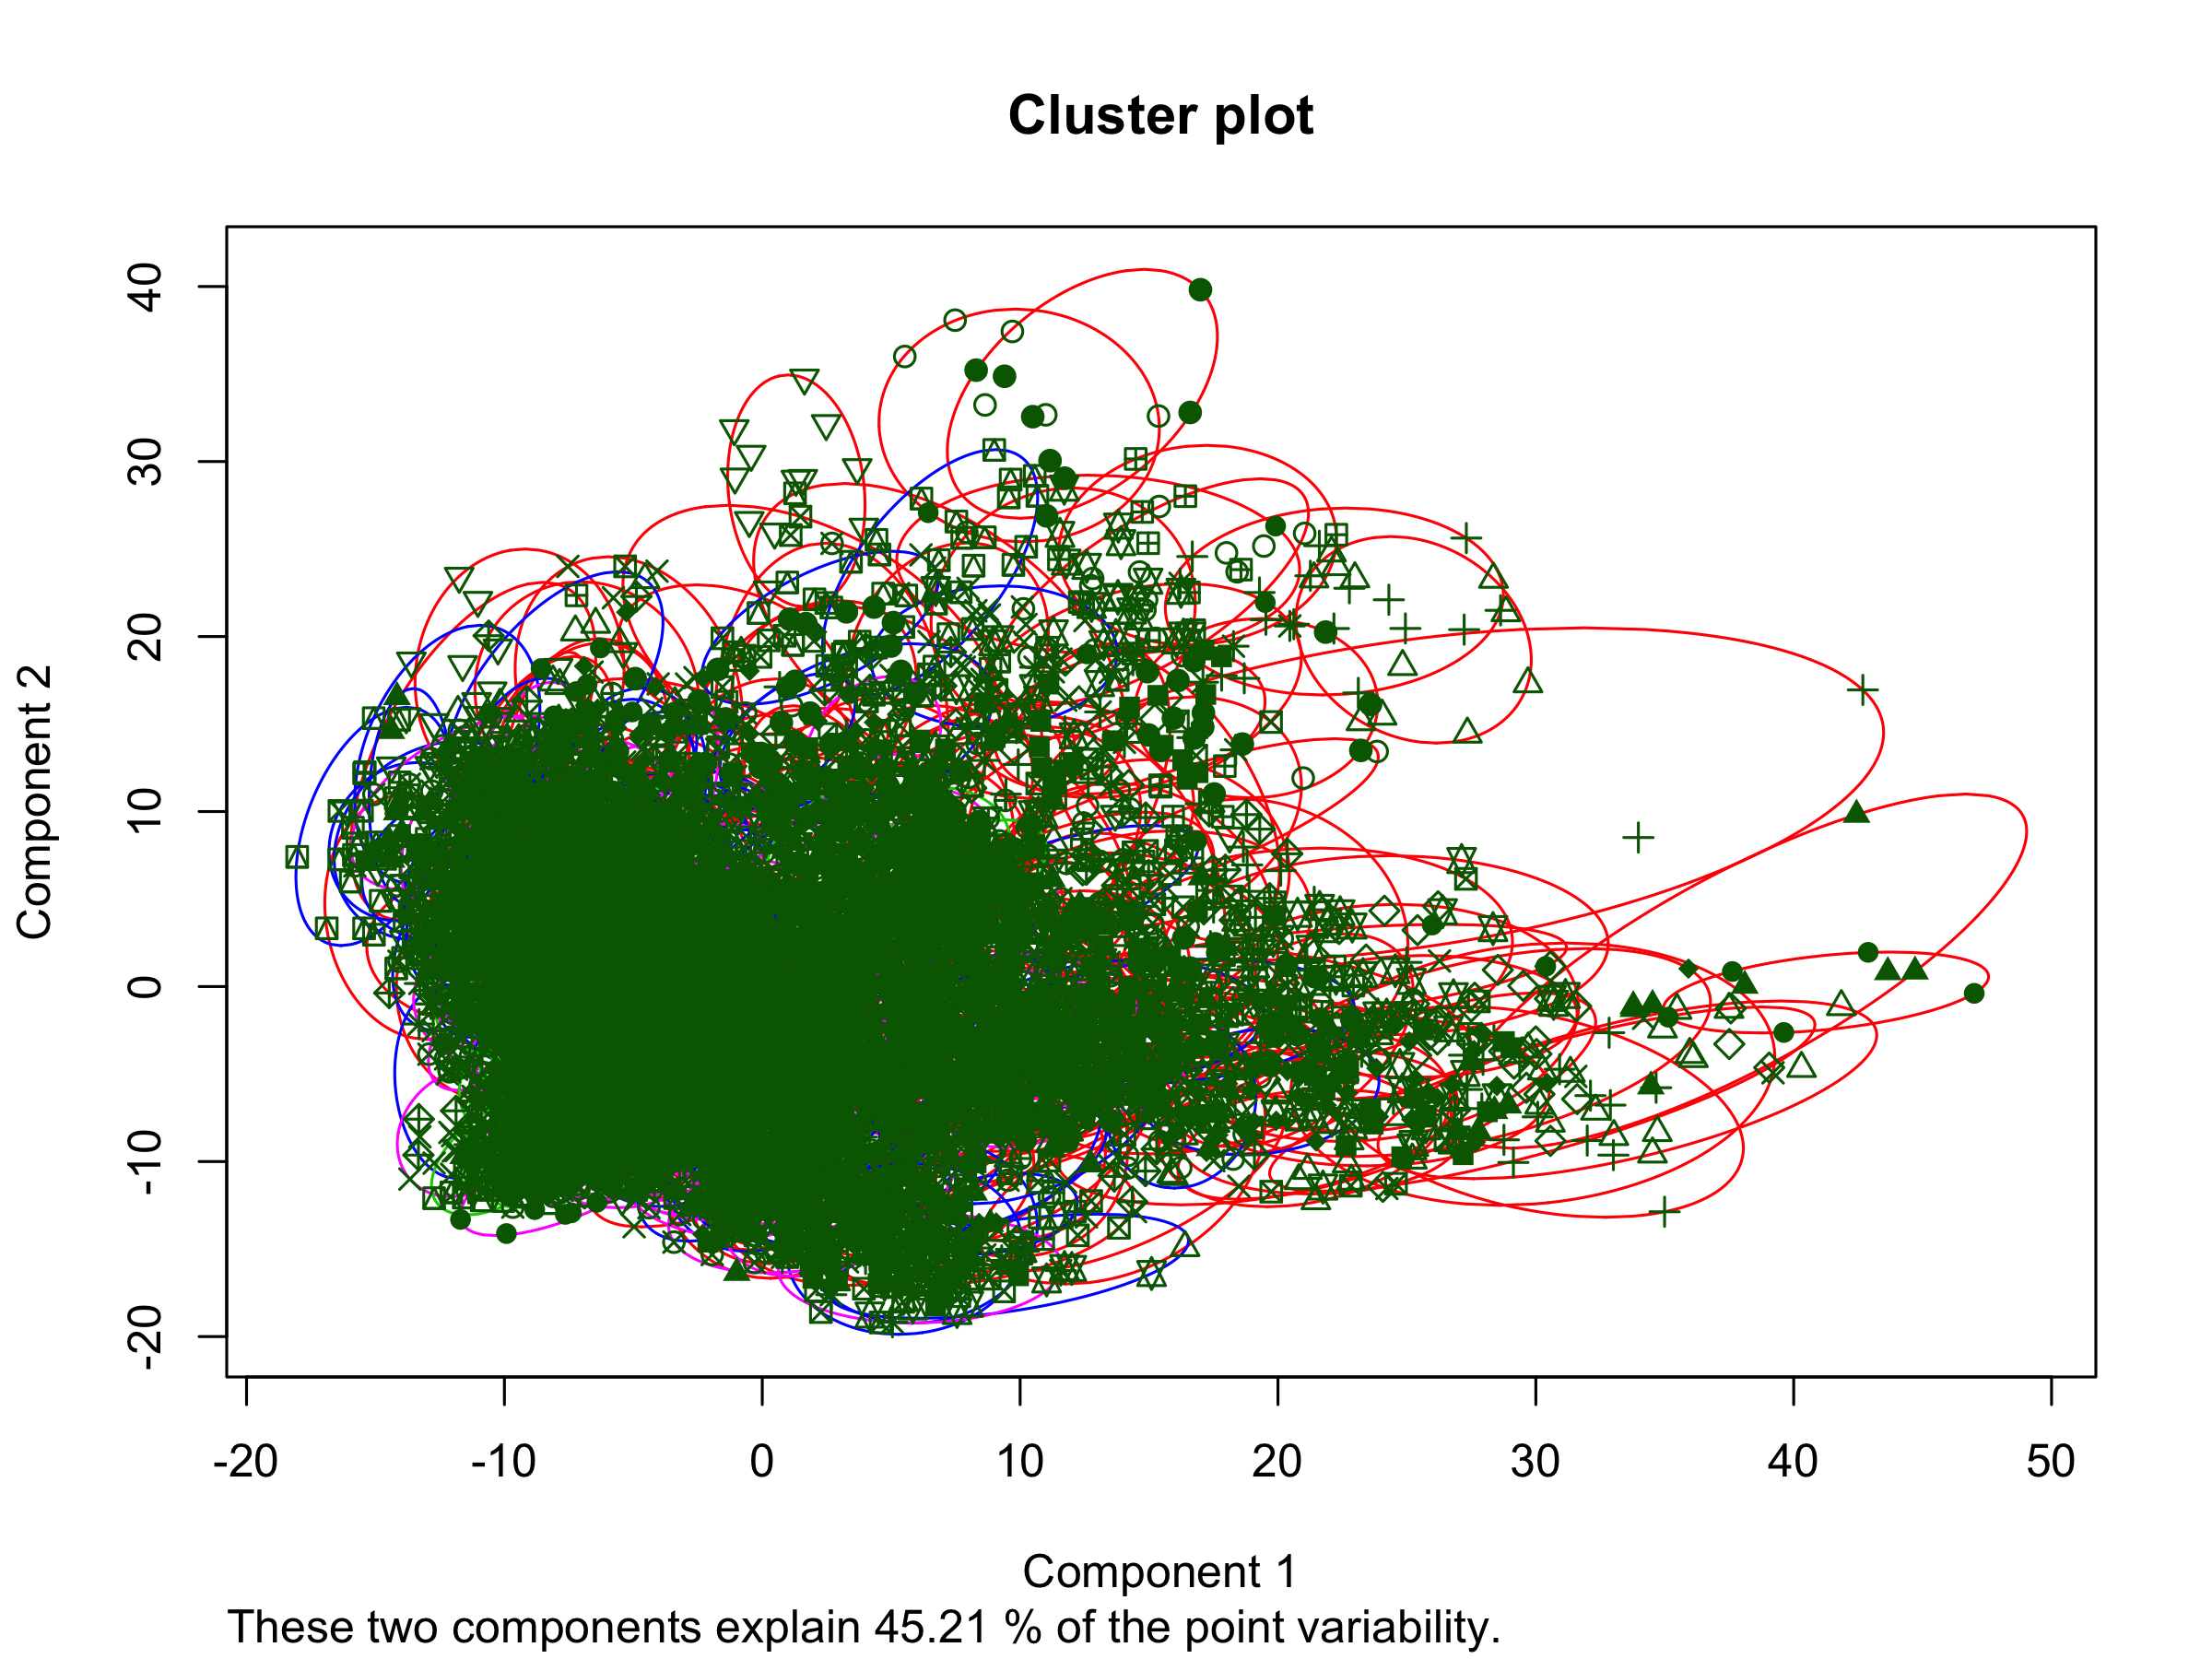
\includegraphics[width = 0.2\textwidth]{clusplot_6.png}\label{fig:6}}\hspace{1em}
%%  		
%%  		
  		\subfloat[Clustering data consiting of digit 7]{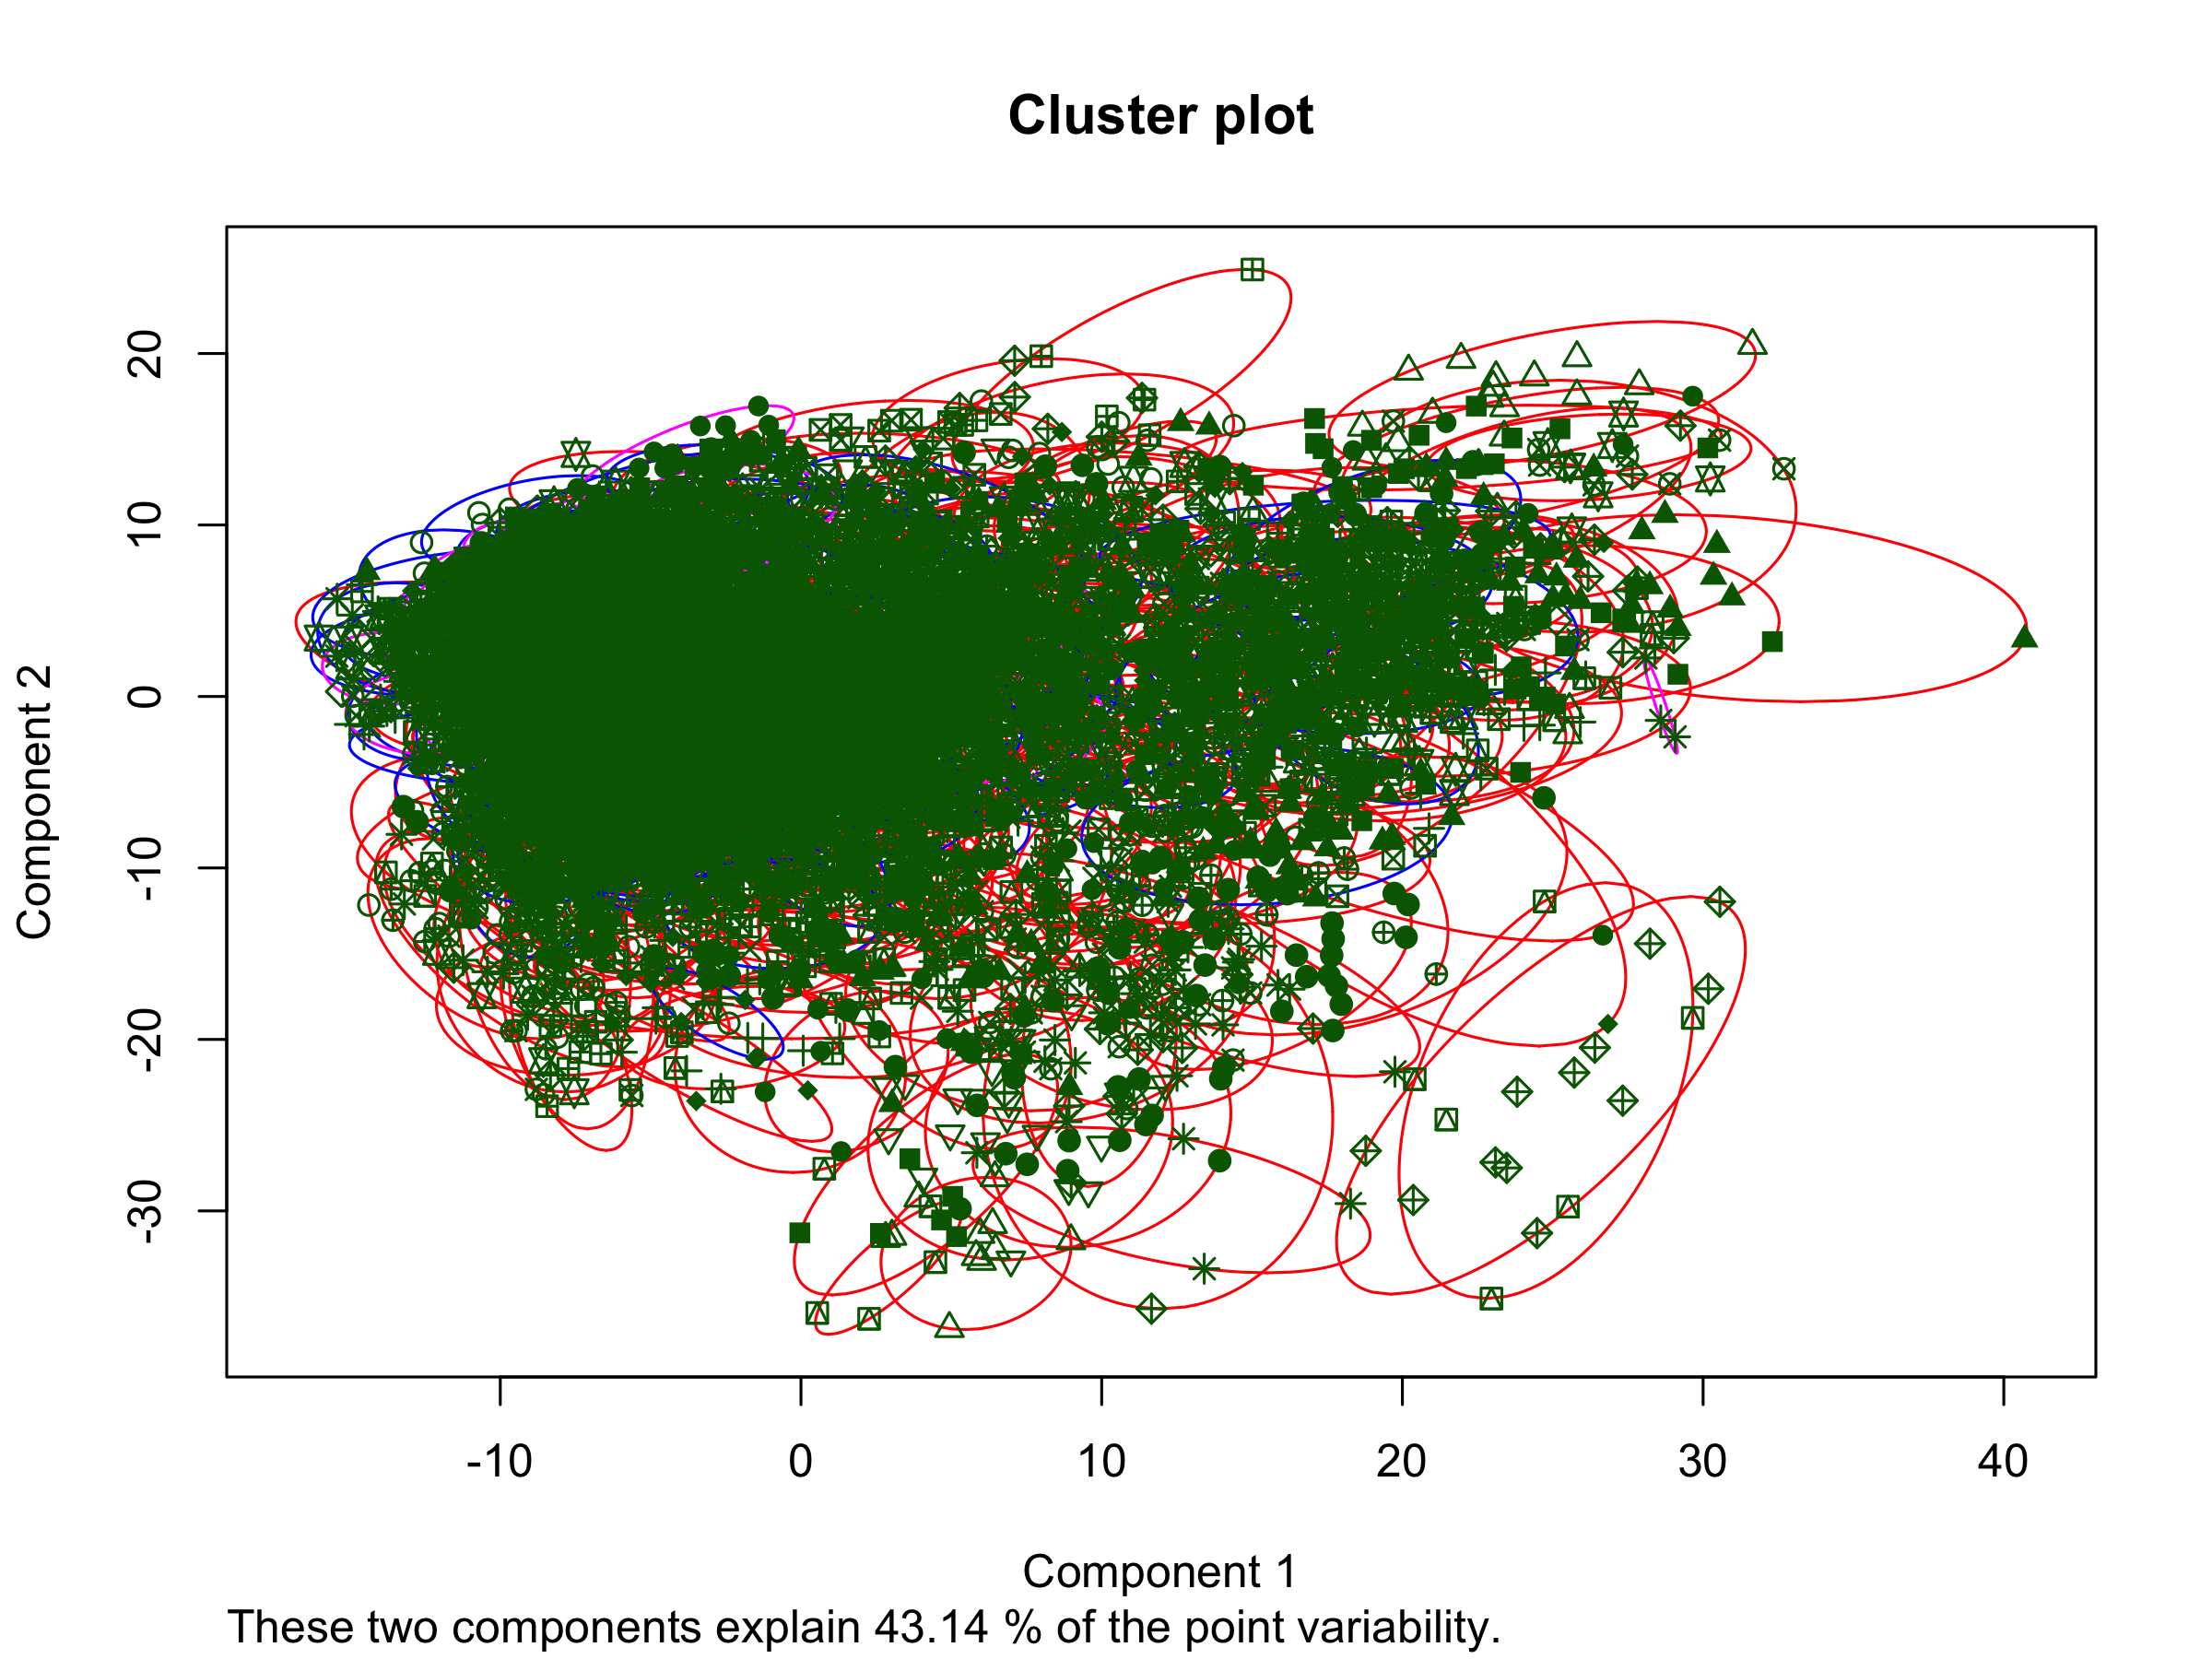
\includegraphics[width = 0.2\textwidth]{clusplot_7.png}\label{fig:7}}
%%
  		\subfloat[Clustering data consiting of digit 8]{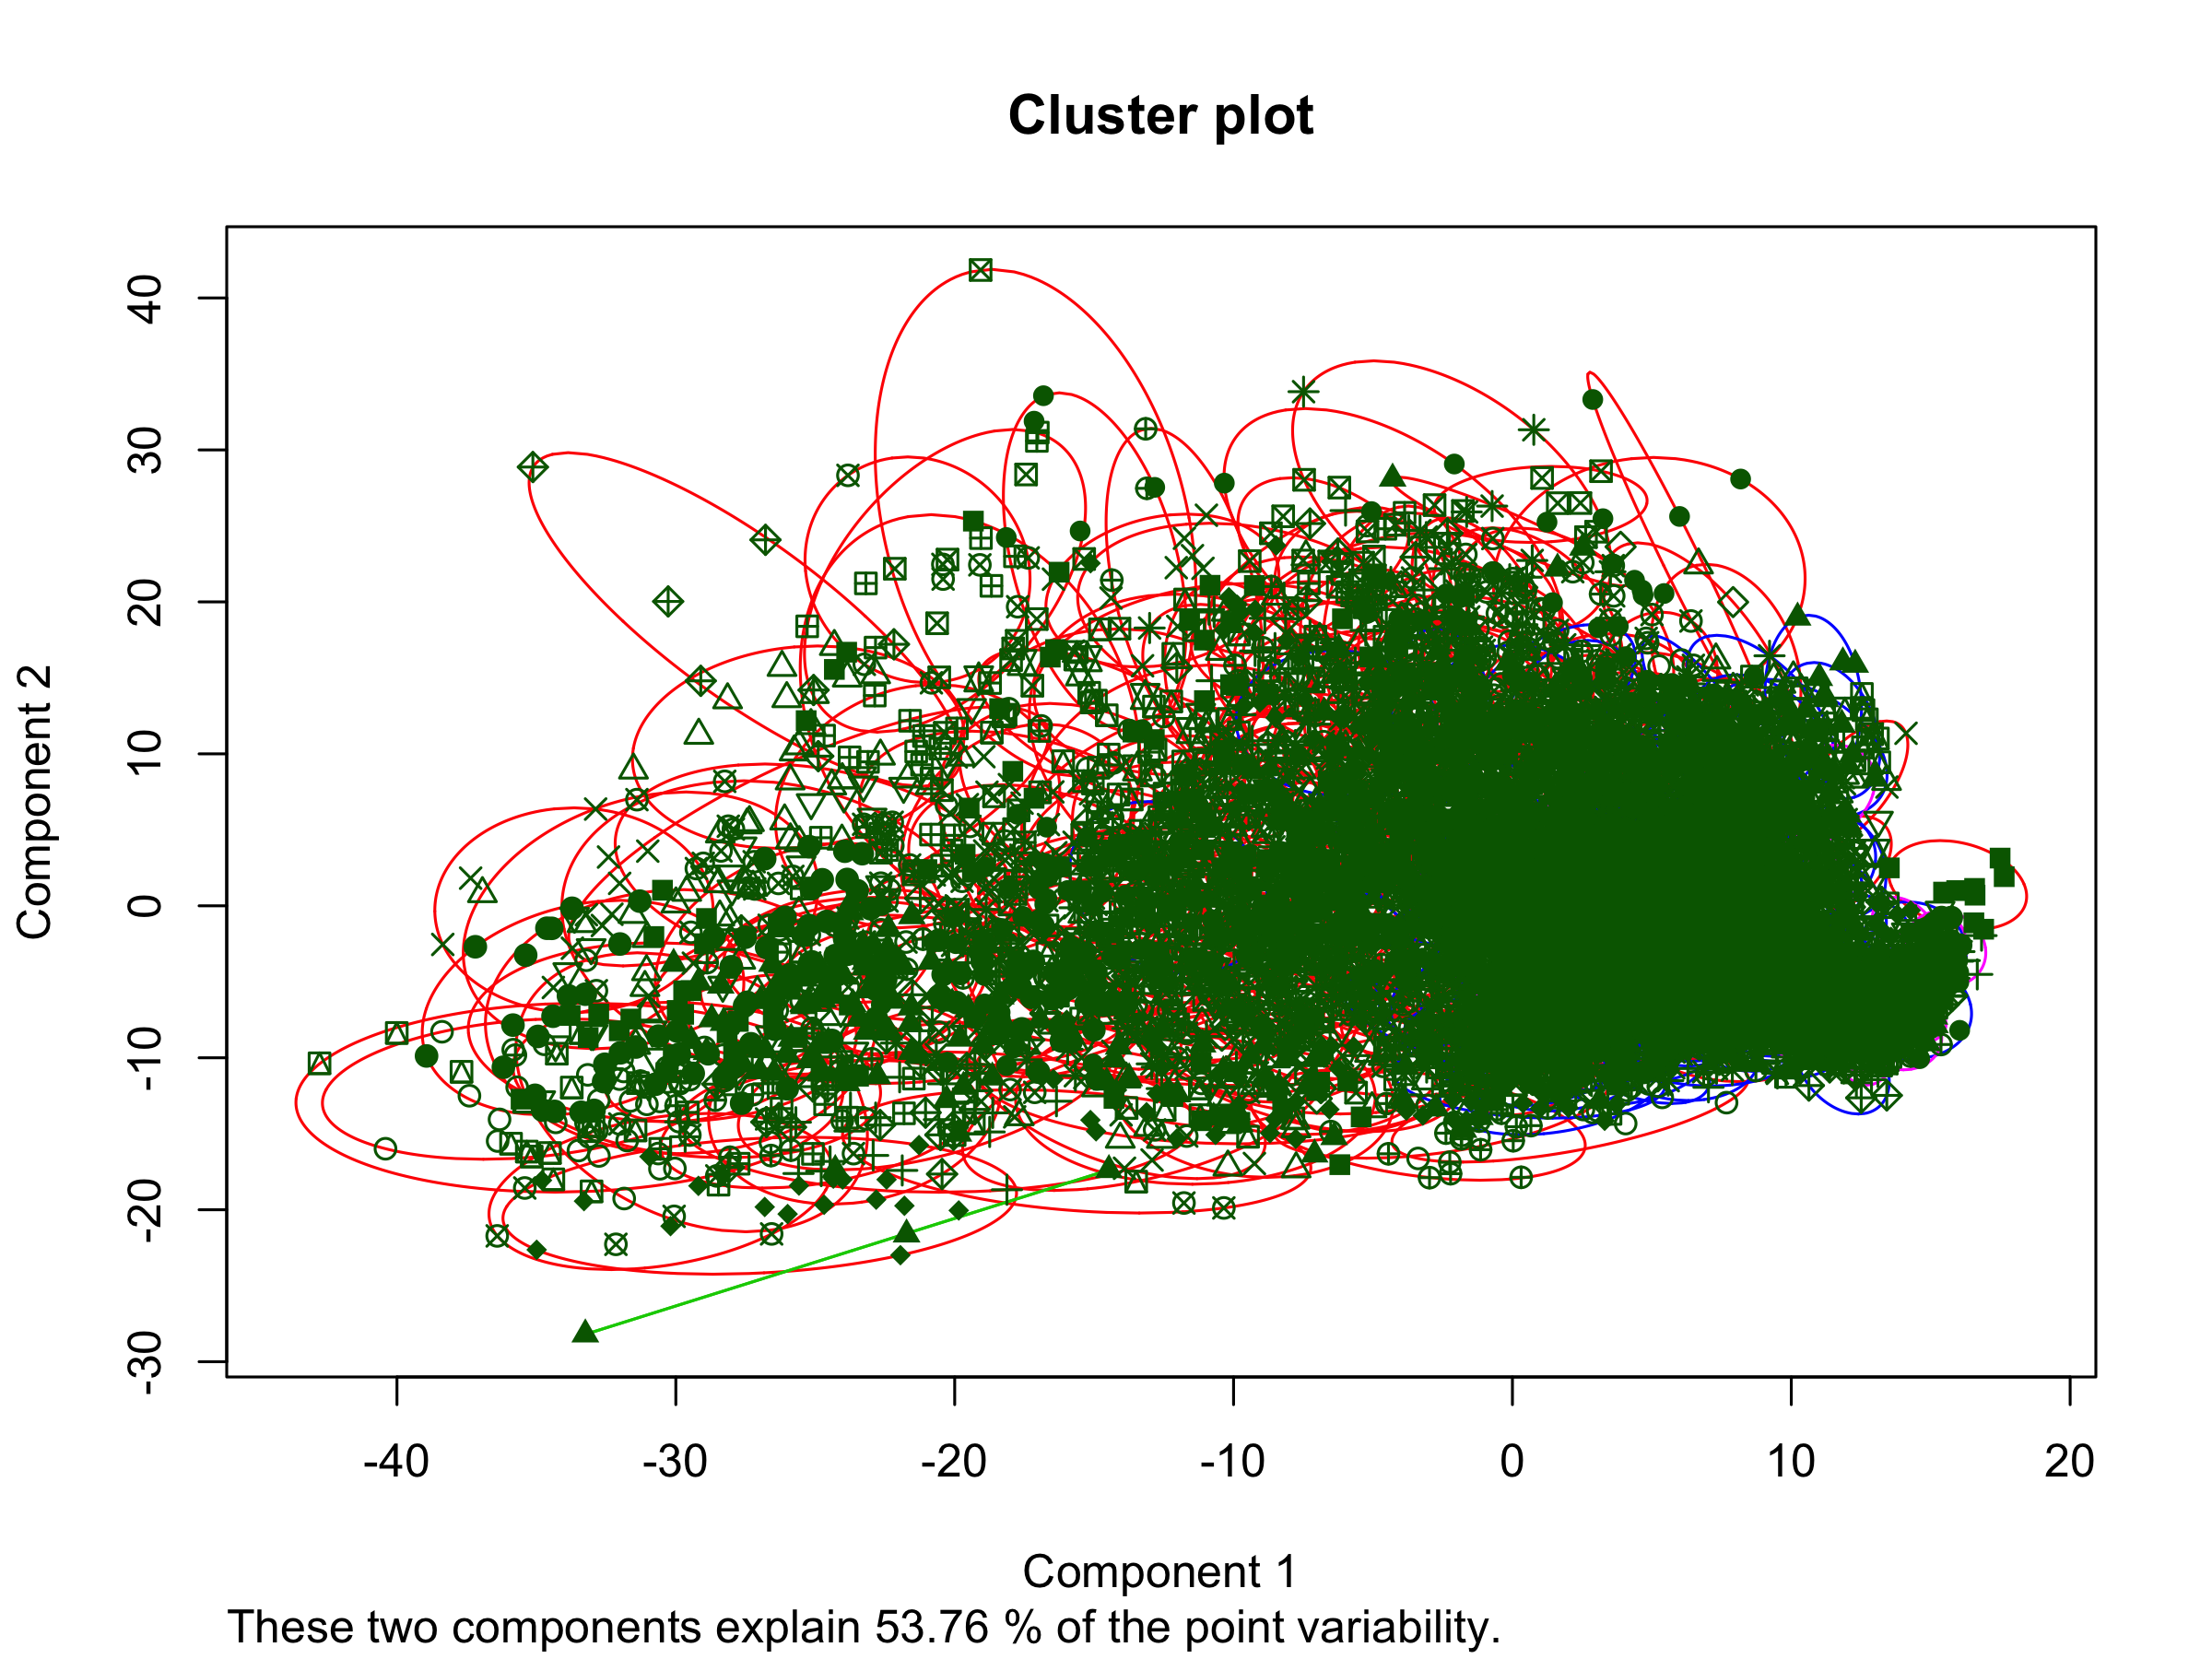
\includegraphics[width = 0.2\textwidth]{clusplot_8.png}\label{fig:8}}
%%  		 
  		 \subfloat[Clustering data consiting of digit 9]{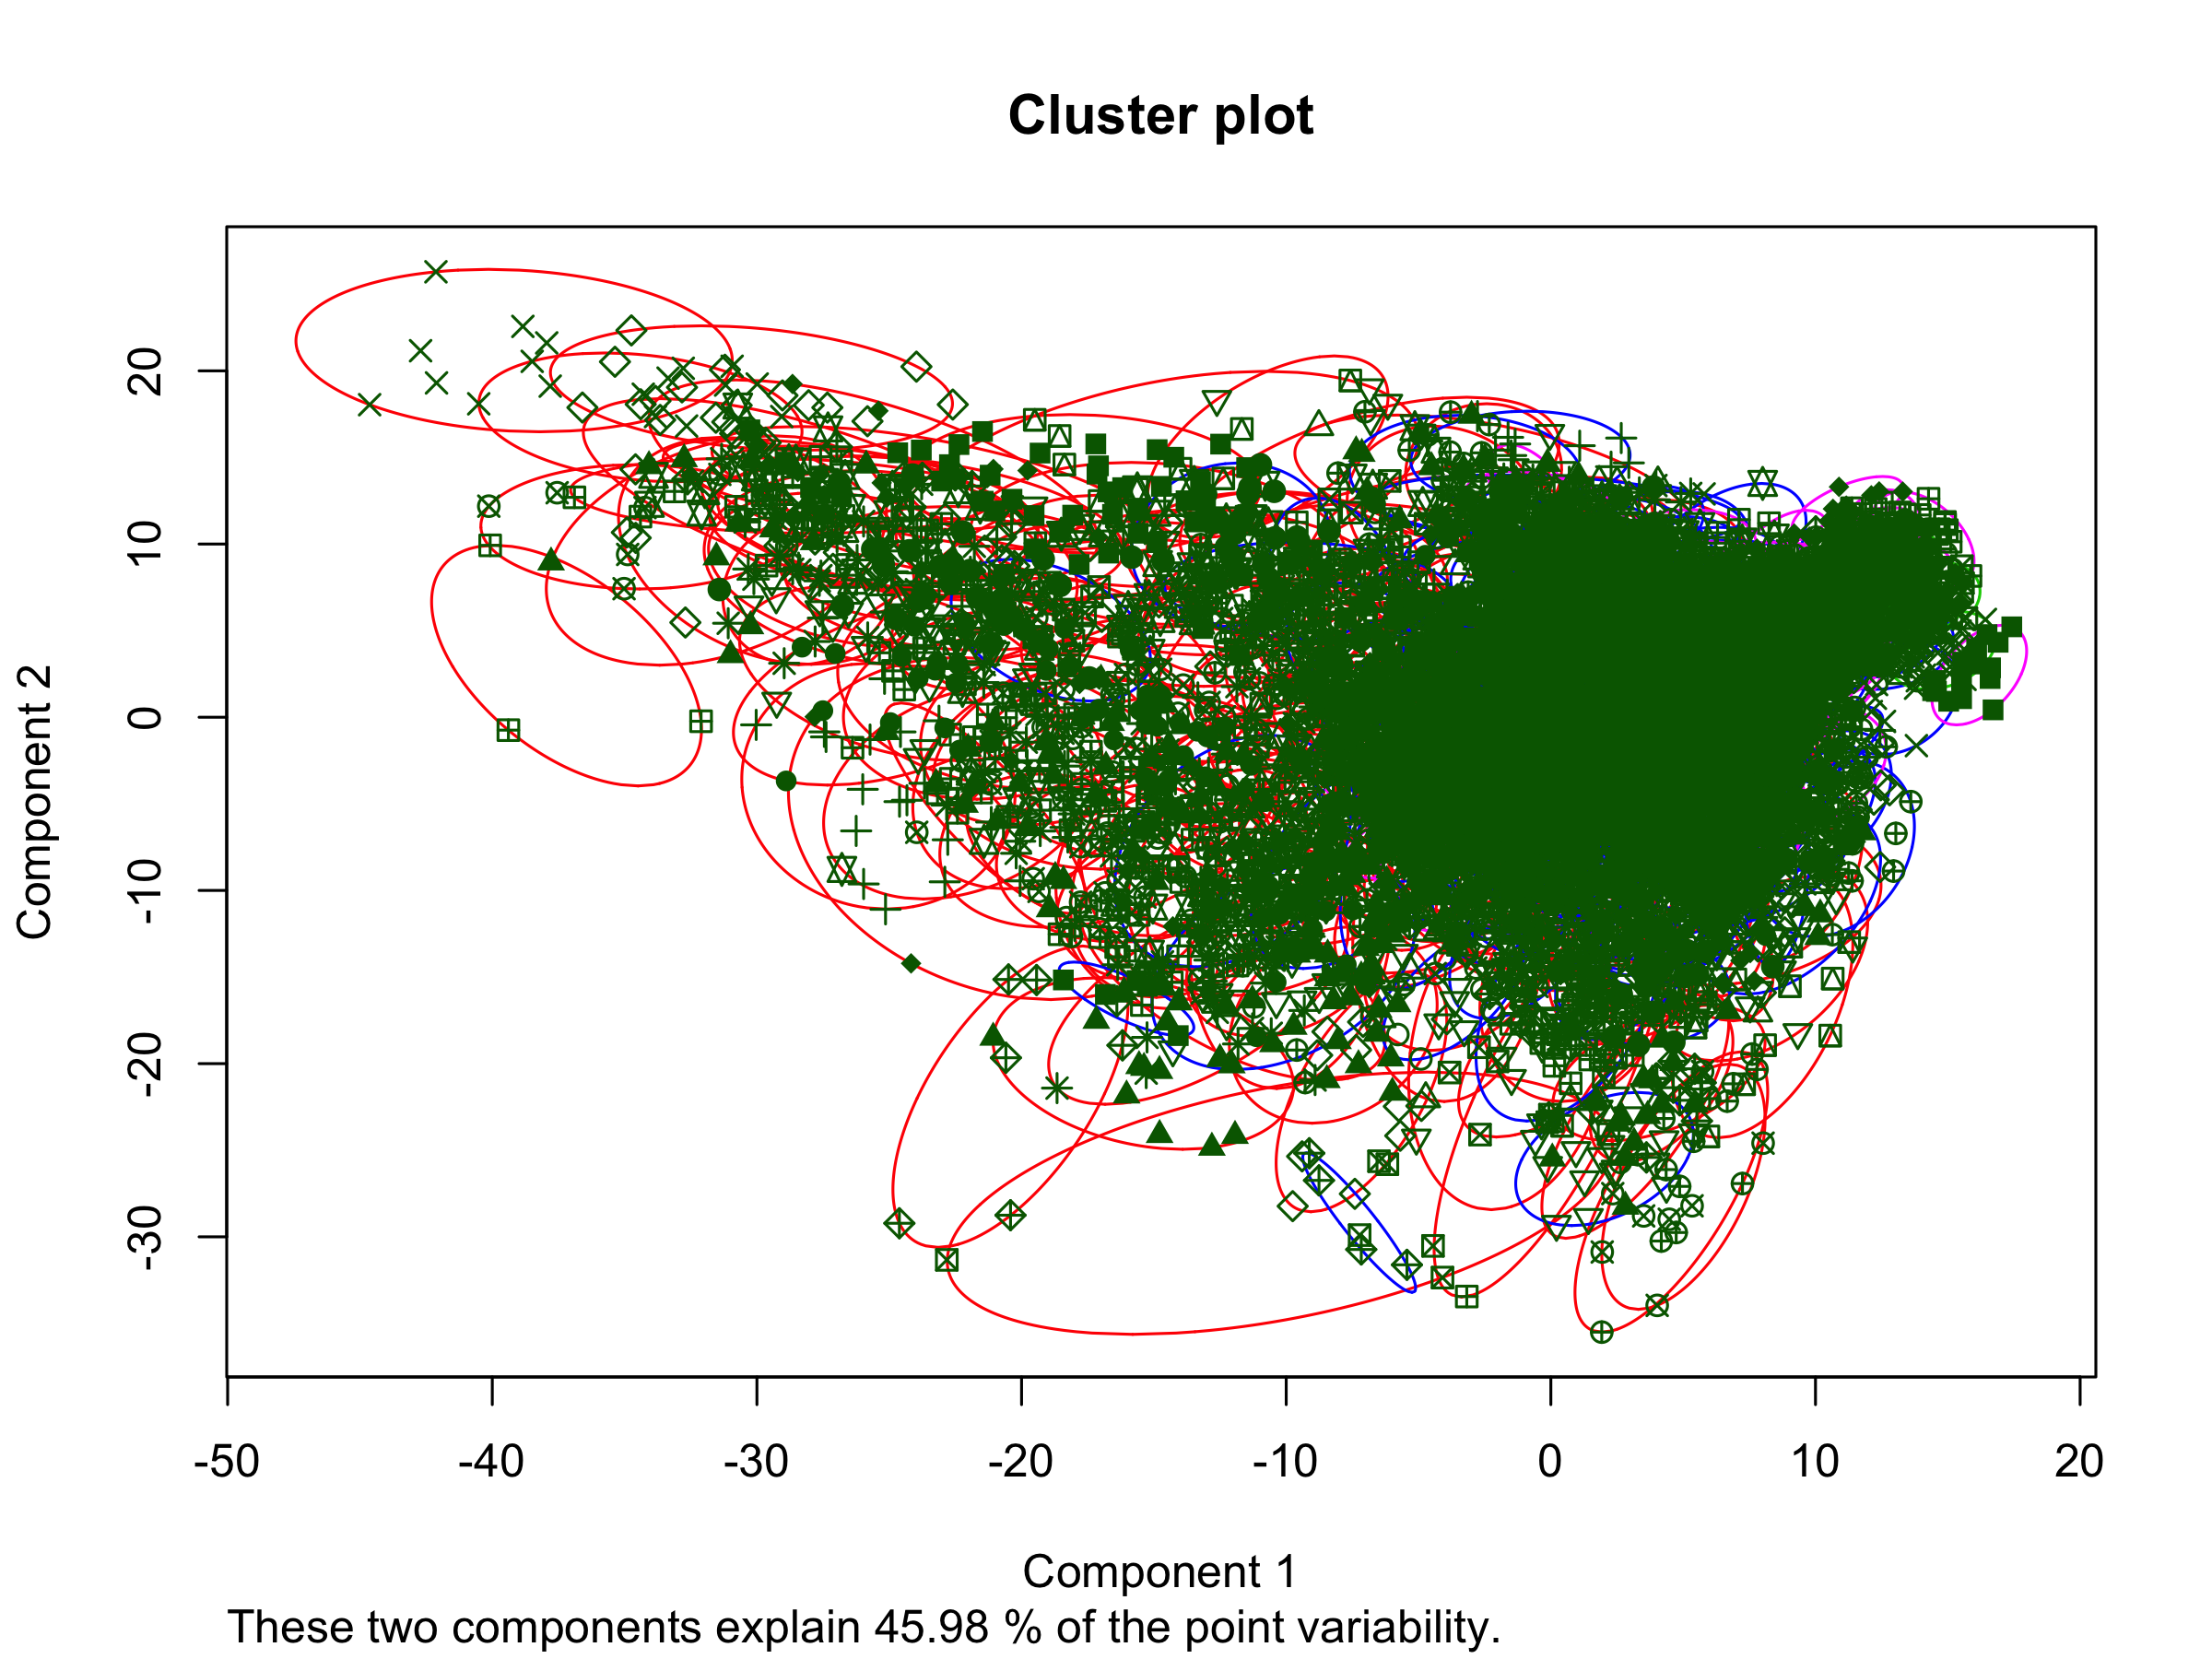
\includegraphics[width = 0.2\textwidth]{clusplot_9.png}\label{fig:9}}\hspace{1em}
  		\caption{This and that}
	\end{figure}


The dendrogram of figure \ref{fig:dendo} visualizes
the digit class clustering, where eg. "X1" represents the digit 1.
Asides from a within-digit similarity, this dendrogram also
hints at a similarity between digits 5 and 6, which,
perhaps, it not surprising as these digits often look similar.

Compared to the confusion matrix of figure \ref{fig:confusionMatrixAll},
the dendrogram quickly groups together a 2 and a 7,
which are among the most often confused digits.
Perhaps this is an indication that too aggressive clustering
will group together examples of different digits
early on, which is an undesired effect of clustering;
It means the number of clusters has to be relatively high
to withstand the similarities between examples of different digits.

\begin{figure}[H]
\label{fig:dendrogram}
		\centering
		 \subfloat[Dendrogram]{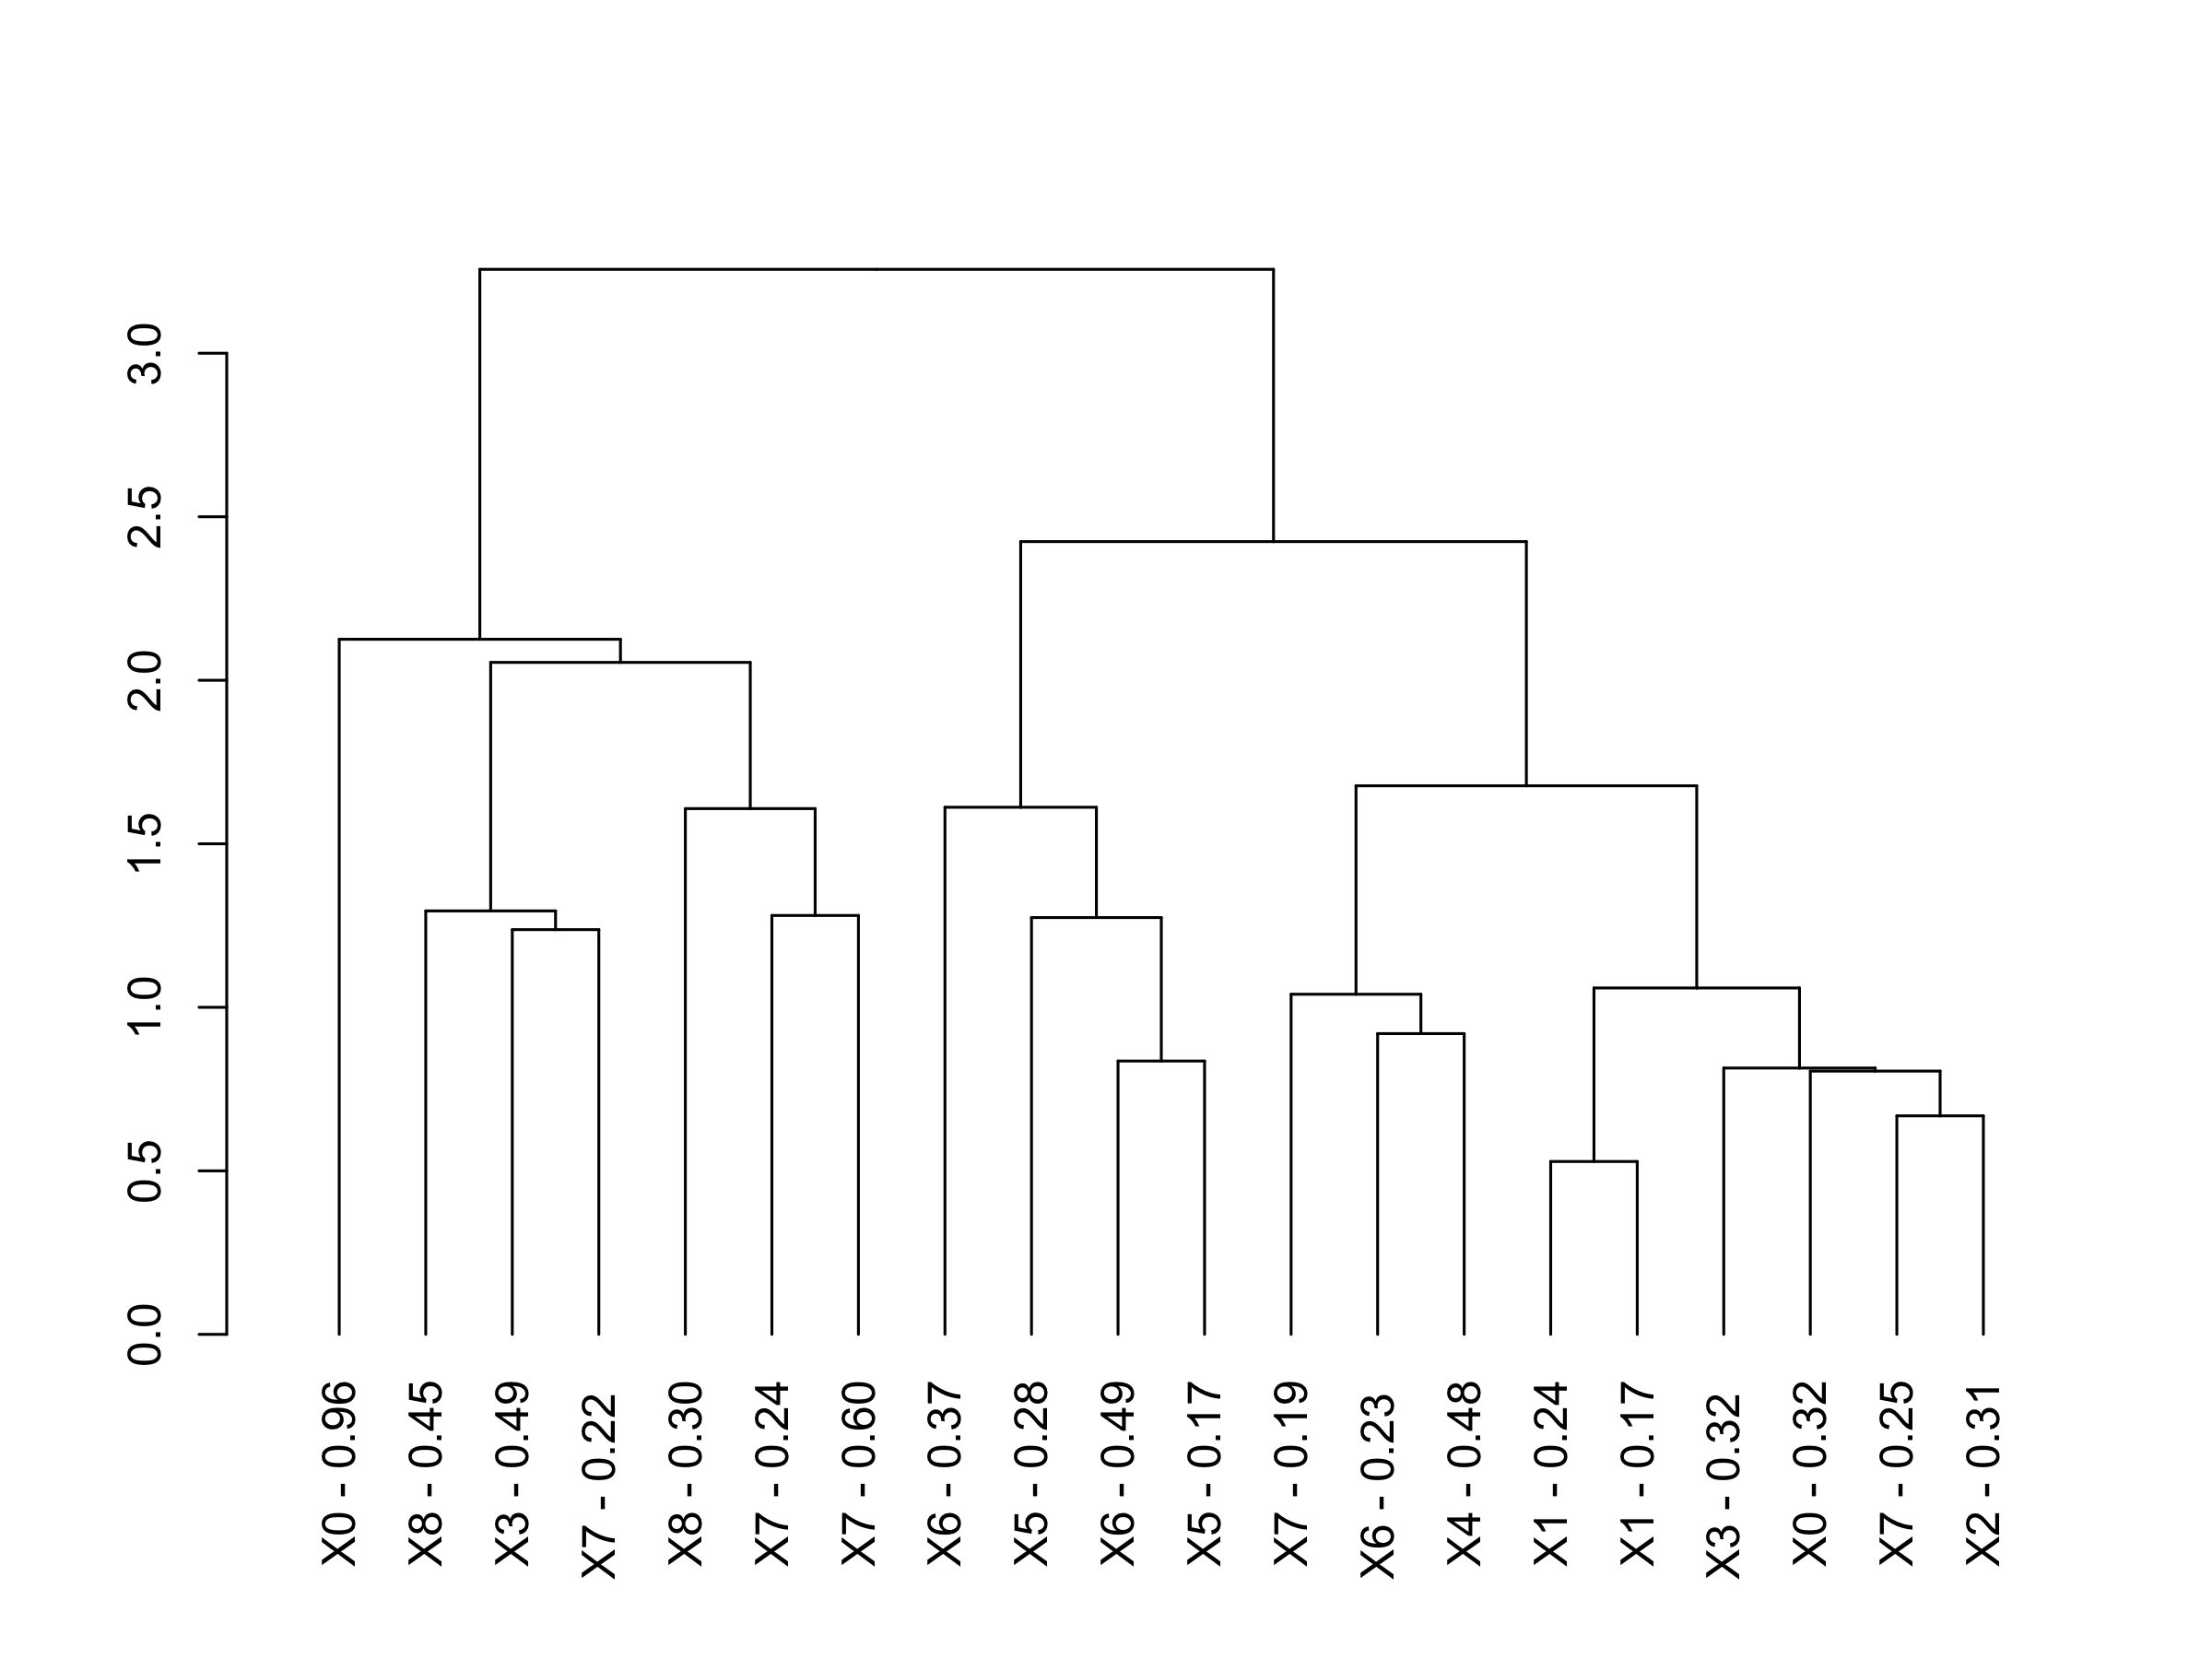
\includegraphics[width = 0.7\textwidth]{dendogram_data_class.png}\label{fig:dendo}} 
\end{figure}																						

\begin{figure}[H]
\label{fig:confusionMatrixAll}
\centering
\subfloat[Confusion matrix]{\includegraphics[width = 0.7\textwidth]{confmatkNN-multiAll-sig15-k1-n40000.eps}}
\end{figure}

		\todo{Insert some test}
		
		
\end{document}